%============================= BACKGROUND =================================

\graphicspath{{img/back/}}

% Often used notations
\renewcommand{\x}{\mathbf{x}} % input vector
\renewcommand{\X}{\mathbf{X}} % input dataset

\renewcommand{\y}{\mathbf{y}} % target/output vector
\renewcommand{\Y}{\mathbf{Y}} % target/output dataset

\renewcommand{\w}{\mathbf{w}} % weight vector
\renewcommand{\W}{\mathbf{W}} % weight matrix
\renewcommand{\b}{\mathbf{b}} % bias vector

\renewcommand{\z}{\mathbf{z}} % aux variable (logits)
\renewcommand{\h}{\mathbf{h}} % hidden state
\renewcommand{\o}{\mathbf{o}} % output variable
\renewcommand{\p}{\mathbf{p}} % vector of probabilities
\renewcommand{\m}{\mathbf{m}} % 1st grad momentum
\renewcommand{\v}{\mathbf{v}} % 2nd grad momentum
\renewcommand{\q}{\mathbf{q}} % query vector

\renewcommand{\i}{\mathbf{i}} % lstm input gate
\renewcommand{\f}{\mathbf{f}} % lstm forget gate
% \renewcommand{\o}{\mathbf{o}} % lstm output gate
\renewcommand{\u}{\mathbf{u}} % lstm update gate
\renewcommand{\c}{\mathbf{c}} % lstm cell state

\renewcommand{\R}{\mathbb{R}} % real numbers
\renewcommand{\L}{\mathcal{L}} % loss function
\renewcommand{\a}{\varphi} % activation function

\renewcommand{\Reg}{\mathcal{R}} % region

\renewcommand{\(}{\left (} % left par
\renewcommand{\)}{\right )} % right par


\chapter{Background}
\label{ch:background}

% TODO add overfit, underfit to background?
% TODO add train good practices? (train/val/test splits, epochs, etc.)

% TODO [+CITE] speech analysis \citep{yan2014age}, object recognition tasks \citep{ciresan2012multi}

In this chapter, we present the basic concepts about \gls{dl}, and we introduce the research fields on which its application has been investigated in this thesis, namely Image Classification and \gls{cbir}.
% TODO add some more intro to the bg chapter?
The chapter is organized as follows.
In \ref{sec:back:deep-learning}, we provide the reader with a quick introduction to \acrlong{dl}, focusing on deep neural networks for image and text processing and gradient-based optimization.
In \ref{sec:back:image-classification}, an introduction to image classification using \acrfullpl{cnn} is presented together with a review of successful approaches in this field.
In \ref{sec:back:image-retrieval}, we describe the main aspects of \gls{cbir} based on image representations extracted from deep neural networks, and we discuss some state-of-the-art methodologies to build effecive description of images and to efficiently index them in large-scale scenarios.
\ref{sec:back:datasets} summarizes the public datasets used in the experiments presented in this thesis.


\section{Deep Learning}
\label{sec:back:deep-learning}

\acrfull{dl} defines a subfield of Artificial Intelligence, specifically of \gls{ml}, in which a \emph{hierarchy of data representations} (or \emph{features}) is learnt from data for solving a particular task~\cite{bengio2007scaling,goodfellow2016deep}.
% TODO add representation learning?, what is and cites
%For historical reasons, \gls{dl} models are also referred to as \emph{\glspl{dnn}} due to the resemblance of layers and their organization to the way neurons are interconnected and organized in the mammalian brain~\cite{}.
% TODO add reference to similarities to mammalian brain (in addition to perceptron?)
Inspired by nature, \acrlong{dl} models are often implemented as \glspl{dnn} --- a computational model comprised by multiple layers of processing units that mimics the structure and the interconnection of neurons in the mammalian brain~\cite{rosenblatt1958perceptron}.
Recent years have witnessed a rapid rise in the use of \gls{dl} approaches to solve complex task, reaching even super-human performance in perceptiual~\cite{he2015delving}, control~\cite{mnih2015human}, and planning~\cite{silver2016mastering} activities. % TODO add reasoning?
Interestingly, the representations learnt with \gls{dl} methodologies resemble the structures of signals in the neocortex build by our brain to implement intelligent behaviours, suggesting a strong parallelism between the two domains~\cite{cadieu2014deep,kubilius2016deep}. % TODO dire meglio?

\acrlongpl{dnn} are organized as a sequence (or more generally a graph) of parametric non-linear transformations, known as \emph{layers}, that acts like features extractors;
starting from raw data, each layer searches for useful patterns in its input and provides higher-level representation of the data to the next layer.

Formally, given an input $\x$, we can express the output $\y$ of \gls{dnn} as
%
\begin{equation} \label{eq:back:deepnet}
    \y & = f\(\x, \Theta\) \,,
%\begin{split}
%    \y & = f\(\x, \Theta\) \\
%       & = f_L\(\dots f_2\(f_1\(\x; \theta_1\); \theta_2\); \theta_L\) \,,
%\end{split}
\end{equation}
%
where $f(\cdot)$ is an arbitrary composition of parametric transformations (layers), and $\Theta$ indicates the set of all the parameters, also known as \emph{weights} of the \gls{dnn}.

Given a training set of input-target couples $\X = \{ (\x_i, \y_i^\star),\; i = 1, \dots, N \}$, the quality of a particular setting of parameters is quantitatively defined by a \emph{loss function} $\L\(\X; \Theta\)$ that measures how much the model predictions $\y$ differ from the targets $\y^\star$ provided by $\X$.
The particular formulation of $\L$ is task-dependent and further discussed in \ref{subsec:back:loss}.
In the end, the learning problem reduces to the optimization problem
%
\begin{equation} \label{eq:back:optim}
    \Theta^\star = \argmin_\Theta \L\(\X; \Theta\) \,,
\end{equation}
%
in which we search the best parameter setting $\Theta^\star$ that minimizes the loss function $\L\(\X; \Theta\)$.

The specific layers used and their interconnections define the \gls{dnn}'s \emph{architecture} (or \emph{computation graph}).
\Glspl{dnn} can be roughly categorized into \glspl{ffnn}, in which information flows from input to output in a non-recursive cascade of computations, and \glspl{rnn}, which present a feedback loop in their computation graph.
In the following sections, we will review some practical and successful formulations of \glspl{dnn},
%that are useful when dealing with image data
and we will provide the reader with the basics of gradient-based optimization of \ref{eq:back:optim}.

\subsection{Feed-Forward Neural Networks}
\label{subsec:back:ffnn}

\Acrlongpl{ffnn} are networks whose computation graph can be expressed as a directed acyclic graph, i.e.\,there are no feedback loops and information flows from inputs to outputs in a cascade fashion.
Thus, when computing of the whole chain from inputs to outputs, called the \emph{forward} pass of the network, each transformation defined by layers is computed only once.

% In the following, we summarize some of the most relevant layers used in \glspl{dnn}.

%\subsubsection{Fully Connected Layer}
\subsubsection{Multilayer Perceptrons}

\begin{figure}
    \includegraphics[ width=\linewidth]{figures/activations}
    \caption{Commonly used activation functions in \glspl{dnn}. The \acrfull{relu} on the left, the sigmoid $\sigma$ in the middle, and hyperbolic tangent on the right.}
    \label{fig:back:activations}
\end{figure}

The \gls{mlp} is the simplest form of artificial neural network in the \Acrlong{dl} field.
A \gls{mlp} is comprised by a cascade of \emph{inner product} (or \emph{fully connected}) layers, which are the basic building block for \glspl{dnn}.
A inner product layer performs a linear projection of the input followed by a usually non-linear element-wise activation function.
Formally, given an input comprised by $n$ features $\x \in \R^n$, the output  $\y \in \R^m$ of the layer is obtained as
%
\begin{equation} \label{eq:back:fully-connected}
    \y = \a \( \W \x + \b \) \,,
\end{equation}
%
where $\W \in \R^{n \times m}$ and $\b \in \R^m$ are learnable parameters of a linear projection to a $m$-dimensional space.
Commonly used activation functions $\a: \R \to \R$ are the \gls{relu}, the sigmoid $\sigma\(\cdot\)$, and $\tanh\(\cdot\)$ functions (depicted in~\ref{fig:back:activations}).
The dimensionality of the input $n$ and of the output $m$ are referred to as respectively the number of \emph{input features} and \emph{output features}.

\begin{figure}
    \centering
    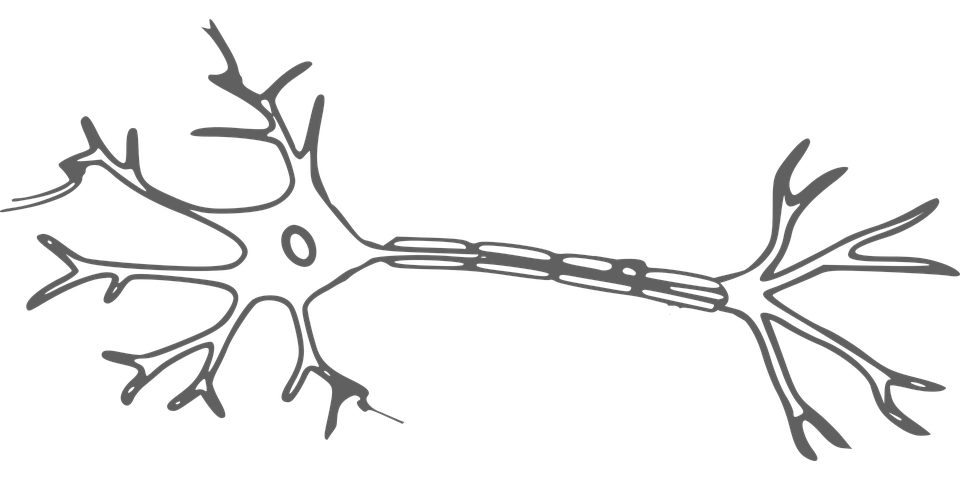
\includegraphics[width=0.8\linewidth]{figures/neuron}
    \caption{Parallelism between a real neuron and the artificial one used in \glspl{mlp}.}
    \label{fig:back:neuron}
\end{figure}

Historically, this layer implemented a group of $m$ \emph{perceptrons}.
The perceptron~\cite{rosenblatt1958perceptron} is a biologically-inspired building block for artificial neural networks that has been developed mimicking the structure of biological neurons (see \ref{fig:back:neuron}).
As a neuron cell, it is composed by $n$ inputs $\x_i$ ($i=1 \dots n$), usually connected to the output of other neurons, and a single output $\mathbf{y}$ (axon).
Each input connection is associated with a weight $\w_i$ ($i=1 \dots n$) expressing how much of the signal coming through that connection is promoted or inhibited.
Weights in a perceptron are interpreted as the strength of the interconnection between neuron cells.
The neuron ``fires'' when the combination of their weighted inputs gets above a certain threshold;
this is modelled in the perceptron defining its output as the activation function $\a(\cdot)$ applied to the inner product between input and weights
%
\begin{equation}
    \y_j = \a \( \sum_{i=1}^n \w_i \x_i + b\) \,,
\end{equation}
%
where $\y_j$ is the output of a particular neuron and $b \in \R$ is an optional weight used as bias term.
% The weight vector $\w$ is tuned in the training phase in order to
A layer composed by $m$ perceptrons (and thus $m$ outputs $\y_j, j=1 \dots m$) sharing the same input $\x$ can be formalized with \ref{eq:back:fully-connected}, where the columns of $\W$ correspond to the weights of the $m$ perceptrons.
% Feed-forward artificial neural networks built stacking layers of perceptrons are called \glspl{mlp}.
In \glspl{mlp}, the outputs of a layer are densely connected to the input of each neuron comprising the next layer, hence the name ``fully-connected layer''.
The output of a \gls{mlp} with $L$ layers is defined as
%
\begin{equation}
    \y = \a \( \W_L \( \dots \a \( \W_2 \( \a \( \W_1 \x + \b_1 \) \) + \b_2 \) \) + \b_L \) \,,
\end{equation}
%
where $\(\W_i, \b_i \)$ are the parameters of the $i$-th fully-connected layer in the network.

\subsubsection{Convolutional Neural Networks}

\begin{figure}
    % TODO [FIG] example of crosscorr on image
    \centering
    \includegraphics[width=0.5\linewidth]{figures/cross-correlation2d}
    \caption{Example of cross-correlation between 2D signals.}
    \label{fig:back:2d-cross-corr}
\end{figure}

A \gls{cnn} is a feed-forward artificial neural network composed by at least one \emph{convolutional} layer.
This kind of layer computes the cross-correlation between the input and a set of learnable filters.
Since there is a strong similarity between the convolution and the cross-correlation operations, this layer is often attributed with the adjective ``convolutional'' in the \gls{dl} literature;
thus we will adopt the same terminology throughout this thesis.

\paragraph{Cross-correlation}
The \emph{cross-correlation} (also called \emph{sliding inner product}) is typically used in signal processing to search for matches between two signals.
Intuitively, a small signal called \emph{filter} containing the prototype we want to match is slided on a bigger input signal, and for each position, the inner product between the intersection of the two signals measures the quality of the match.
We will provide the reader with the formulation of the two-dimensional version of the cross-correlation due to its massive adoption in image-related fields that are of interest for this work.

Given a two-dimensional input matrix $\x \in \R^{H \times W}$ and a two-dimensional filter $\w \in \R^{K_1 \times K_2}$, %with $K \ll \min(H,W)$,
the cross-correlation $\y \in \R^{H' \times W'}$ between $\x$ and $\w$ is given by
%
\begin{equation}\label{eq:back:cross-correlation}
    \y_{u,v} = \sum_{i=1}^{K_1} \sum_{j=1}^{K_2} \w_{i,j} \x_{i+u-1,j+v-1} \,,
\end{equation}
%
where $u = 1, \dots, H'$ and $v = 1, \dots W'$.
Intuitively, the filter $\w$ is superimposed on the input $\x$, and for each possible position $(u,v)$, the scalar product between the covered input and the filter is computed.
Depending on the presence of padding $P$ added to each side of the input and the stride $S$ of the filter application, the output dimensionality changes following the relations
\begin{equation} \label{eq:back:conv-size}
\begin{split}
    H' = \left \lfloor \frac{H + 2 \times P - K_1}{S} \right \rfloor + 1 \,,\quad
    W' &= \left \lfloor \frac{W + 2 \times P - K_2}{S} \right \rfloor + 1 \,.
\end{split}
\end{equation}
Inputs and outputs of convolutional layers are also called \emph{feature maps}, since high values in the two-dimensional map are usually interpreted as the presence of a feature a particular filter has learnt to identify.
A depiction of 2D cross-correlation is reported in~\ref{fig:back:2d-cross-corr}.

\begin{figure}
    \centering
    \includegraphics[width=\linewidth]{figures/convolution}
    \caption{Depiction of 2D cross-correlation on volumes implemented in convolutional layers.}
    \label{fig:back:convolution}
\end{figure}

\paragraph{2D Cross-correlation on Volumes}
\ref{eq:back:cross-correlation} defines the cross-correlation operation for inputs and outputs having both a single feature map.
Images instead are represented as 3-D tensors having $C$ channels (e.g.\ $C=3$ for RGB data, $C=1$ for grayscale) and two spatial dimensions $H$ and $W$;
thus, the definition of the 2D cross-correlation is extended to 3D tensors letting the filters span the depth of the input tensor.
In such way, filters are still applied over the two spatial dimensions $H$ and $W$, but each output value depends on all the input feature maps in a particular spatial position.
Formally, given an input tensor $\x \in \R^{H \times W \times C}$ and a filter $\w \in \R^{K_1 \times K_2 \times C}$ the cross-correlation $\y \in \R^{H' \times W'}$ between $\x$ and $\w$ is defined as
%
\begin{equation}\label{eq:back:channel-cross-correlation}
    \y_{u,v} = \sum_{i=1}^{K_1} \sum_{j=1}^{K_2} \sum_{k=1}^C \w_{i,j,k} \x_{i+u-1,j+v-1,k} \,.
\end{equation}

A convolution layer is often composed by a bank of $K$ filters.
Each filter is applied to the input, obtaining $K$ output feature maps that are stacked along the depth dimension.
The obtained output is a new 3D tensor $\y \in \R^{H' \times W' \times K}$ that is commonly followed by an element-wise non-linear activation $\a(\cdot)$.
The entire process is depicted in \ref{fig:back:convolution}.

The main difference between fully-connected layers and convolutional layers is the way weights are utilized;
while fully-connected layers have a dedicated weight for each couple of input and output features, a convolutional layer shares the weights of its filters across the spatial dimensions, thus learning to detect translation-invariant features by design.

\paragraph{Pooling Layers}
Pooling layers are often used in \glspl{cnn} to reduce the amount of data to be processed in the next layers.
As the name suggests, this kind of layers pools data in groups and aggregates them using a non-parametric aggregation function, such as maximum or average.
The groups are defined as fixed-size windows that are slided along one or more dimensions of the data in the same way the cross-correlation operator is applied.
In the two-dimensional case, input and output sizes follow \ref{eq:back:conv-size}.
The application of convolutional layers having small strides usually produce redundant local information in their output.
Thus, a max-pooling layer is often used to reduce the resolution of intermediate feature maps.
% Instead, sum- and average-pooling are used to produce

\paragraph{Features hierarchy in \glspl{cnn}}
Convolutional layers are stacked to build deep \glspl{cnn}, that are the one of the core tools of Deep Learning for image perception and analysis~\cite{krizhevsky2012imagenet,sermanet2013overfeat,simonyan2014very,he2015delving,he2016deep,xie2017aggregated}.
Once trained, filters in a deep \gls{cnn} tend to organize in a hierarchy of detectors, where layers near the input detect the presence of simple features in the input data, while the following layers build up from them and detect more complex features.
A successful example of the representative power of \glspl{cnn} is object recognition.
% TODO [CITE] object hierarchical decomposition
The visual aspect of objects in images follow a hierarchical organization: an object can be decomposed in parts, parts in patches, patches in textures, textures in edges or blobs, and finally in pixels~\cite{}.
\begin{figure}
    % TODO [KEEP?] is feat hier figure valuable?
    \centering
    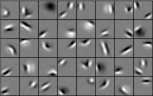
\includegraphics[height=2.9cm]{feat-hier-1.png}%
    \hfill%
    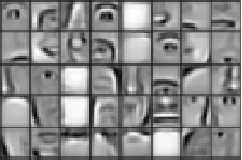
\includegraphics[height=2.9cm]{feat-hier-2.png}%
    \hfill%
    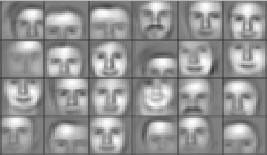
\includegraphics[height=2.9cm]{feat-hier-3.png}%
    \newline
    \caption{
    Visualization of the feature hierarchy learned by convolutional layers in a \gls{dl}-model trained on faces.
    Low-level features (edges and blobs, on the left) are detected and then combined to recognize parts (eyes, nose, mouth, in the middle) and finally faces (on the right).
    \figfrom{lee2011unsupervised}.
    }
    \label{fig:back:filter-hier}
\end{figure}
\Glspl{cnn} trained to recognize objects, directly or indirectly, often organize their hierarchy of detectors following this kind of visual decomposition of objects (see \ref{fig:back:filter-hier}).


\subsection{Recurrent Neural Networks}
\label{subsec:back:rnn}

A \acrfull{rnn} is a stateful artificial neural network with feedback connections in which the output depends not only on the input, but also on the current state of the network~\cite{goodfellow2016deep,rumelhart1986learning}.
The state of the network acts as a memory which is updated at each input, allowing information to persist between inputs.
This architecture is naturally able to process sequences of inputs;
the elements of a sequence can be fed to the network one by one, updating the internal state of the network to compactly represent the sequence processed so far regardless of its length.
% This is achieved by adding a cycle in the computation graph ---

\begin{figure}
    \centering
    \includegraphics[width=.9\linewidth]{figures/rnn}
    \caption{Basic architecture of a \acrlong{rnn} (left). On the right, its unrolled version for a sequence of length 5.}
    \label{fig:back:rnn}
\end{figure}

Given a sequence of inputs of length $T$ $\x_t \in \R^n, t = 1 \dots T$, and an initial state $\h_0 \in \R^m$, a \gls{rnn} can be described as a parametric function mapping the input and the state at a certain timestep to the next hidden state
%
\begin{equation}\label{eq:back:rnn}
    \h_t = f\(\x_t, \h_{t-1}; \W\) \,,
\end{equation}
%
where $f(\cdot)$ is the \emph{recurrent cell} of the \gls{rnn} parametrized by the weights $\W$, and $\h_t \in \R^m, t = 1 \dots T$ is the hidden state at timestep $t$, i.e.\ the state of the network after all inputs until $\x_t$ have been processed.
In its simplest form, the recurrent cell $f$ can be implemented using a fully-connected layer that operates
on the concatenation of the current state and input
%
\begin{equation}
    \h_t = \W [ \x_t | \h_{t-1} ] + \b \,,
\end{equation}
%
where $\W$ and $\b$ are the parameters of a fully-connected layer, and $[\cdot|\cdot]$ is the concatenation operation.
During learning, the \gls{rnn} is unrolled in time to the length of the input sequence to create an acyclic computation graph similar to \glspl{ffnn} (see \ref{fig:back:rnn}) on which standard training procedures can be applied (that will be discussed in \ref{subsec:back:optim}).
Depending on the task we want to model, we could be interested in the last hidden state $\h_T$ compactly represent the whole sequence, or we could use a combination of all hidden states $\h_i, i=1 \dots T$ to get access to the evolution of the information processed through time.

\paragraph{Bidirectional \glspl{rnn}}
In many tasks --- such as sequence classification and segmentation --- also the future context of the sequence is informative. However, \ref{eq:back:rnn} defines a \gls{rnn} encoding only past information, i.e.\   $\h_t$ depends only on information at time step $t' < t$.
To overcome this limitation, \emph{bidirectional} \glspl{rnn} have been proposed~\cite{schuster1997bidirectional}.
Bidirectional architectures adds a separate recurrent cell which process the sequence in reverse order (from future to past)
%
\begin{equation}
    \h'_t = f'\(\x_t, \h'_{t+1}; \W'\) \,,
\end{equation}
%
where $\h'_t$ encodes the "future" part of the sequence, i.e.\ depends on information at time step $t' > t$.
The concatenation of the internal states of both past-to-future and future-to-past \glspl{rnn} $[\h_t | \h'_t]$ is often used as the representation of the whole sequence.

\begin{figure}
    \centering
    \includegraphics[width=.9\linewidth]{figures/bidir-rnn}
    \caption{Unrolled version of a Bidirectional \gls{rnn} for a sequence of length 5.}
    \label{fig:back:bidir-rnn}
\end{figure}

\subsubsection{Long Short-Term Memory}

\Gls{lstm}~\cite{hochreiter1997long} is a type of \gls{rnn} with a special formulation of the recurrent cell that has proved its effectiveness in several sequence-modeling tasks~\cite{graves2013speech,sutskever2014sequence,donahue2015long,vinyals2015show}.
This particular formulation is aimed at solving some major drawbacks of vanilla \glspl{rnn}, most importantly the inability to encode long-term dependencies in long sequences due to gradient instability problems, namely the problem of vanishing or exploding gradients ~\cite{pascanu2013difficulty}.
\Gls{lstm} cells are comprised by four learnable gating functions that better control the evolution of the internal state of the cell when dealing with long sequences, and mitigating problems occurring in vanilla RNNs, such as vanishing gradients~\cite{bayer2015learning}.

Let $\x_t \in \R^n$ an element of a sequence, and $\h_{t-1} \in \R^m$ the current hidden state.
The \emph{forget} gate $\f_t$ decides which information is to be discarded at the current step, and it is implemented as a fully-connected layer with $p$ output features and parameters $\w_f \in \R^{(n+m)\times p}, \b_f \in \R^p$ followed by a sigmoid activation
\begin{equation*}
    \f_t = \sigma\(\w_f [\h_{t-1} | \x_t] + \b_f\) \,.
\end{equation*}
The input gate $\i_t$ encodes the information that need to be inserted in the internal state of the cell $\c_t$, and it is implemented following the same rationale of the previous gate
\begin{equation*}
    \i_t = \sigma\(\w_i [\h_{t-1} | \x_t] + \b_i\) \,.
\end{equation*}
The update gate $\u_t$ modulates the amount of new input to be inserted in the internal state of the cell $\c_t$
\begin{equation*}
    \u_t = \tanh\(\w_u [\h_{t-1} | \x_t] + \b_u\) \,.
\end{equation*}
The new cell state $\c_t \in \R^p$ is computed as the sum of two terms;
the first one, given by the element-wise product ($*$) between the forget gate and the previous cell state, represents the part of the old state not to be forgotten;
the second one, computed as the element-wise product of the input and update gates, represent the modulated input to be kept in the new state;
\begin{equation*}
    \c_t = \f_t * \c_{t-1} + \i_t * \u_t \,.
\end{equation*}
The output gate $\o_t$ decides which information in the cell needs to be transferred to the final state $\h_t$
\begin{equation*}
    \o_t = \sigma\(\w_o [\h_{t-1} | \x_t] + \b_o\) \,,
\end{equation*}
and finally, the output state $\h_t$ is computed as
\begin{equation*}
    \h_t = \o_t * \tanh\(\c_t\) \,.
\end{equation*}
%
With an abuse of notation, the complete \gls{lstm} formulation can be compactly written as follows:

%\begin{align}\label{eq:back:lstm}
    % \begin{pmatrix} \i_t\\ \f_t \\ \o_t \\ \u_t \end{pmatrix}
%    \i_t &= \sigma\(\W_i [\h_{t-1} | \x_t] + \b_i\) \\
%    \f_t &= \sigma\(\W_f [\h_{t-1} | \x_t] + \b_f\) \\
%    \o_t &= \sigma\(\W_o [\h_{t-1} | \x_t] + \b_o\) \\
%    \u_t &= \tanh\(\W_u [\h_{t-1} | \x_t] + \b_u\) \\[2ex]
%    \c_t &= \f_t * \c_{t-1} + \i_t * \u_t \\
%    \h_t &= \o_t * \tanh\(\c_t\)
%\end{align}
\begin{align}\label{eq:back:lstm}
\begin{aligned}
    \begin{pmatrix} \i_t\\ \f_t \\ \o_t \\ \u_t \end{pmatrix} &=
    \begin{pmatrix} \sigma \\ \sigma \\ \sigma \\ \tanh \end{pmatrix}
    \( \W \begin{pmatrix} \x_t \\ \h_{t-1} \end{pmatrix} \) \\[2ex]
    \c_t &= \f_t * \c_{t-1} + \i_t * \u_t \\
    \h_t &= \o_t * \tanh\(\c_t\) \,,
\end{aligned}
\end{align}
%
where $\W \in \R^{(n+m) \times 4p}$ summarizes all the parameters of all the fully-connected layers forming the gates.
% TODO: [FIG] lstm?
A depiction of the \gls{lstm} cell is aslo available in \ref{fig:back:lstm}.

\begin{figure}
    \centering
    \includegraphics[width=\linewidth]{figures/lstm}
    \caption{Example of \gls{lstm} cell.}
    \label{fig:back:lstm}
\end{figure}

\subsection{Loss Functions}
\label{subsec:back:loss}

Loss functions are a key component of \gls{ml} methods.
Its role is to quantitatively assign a value of goodness to a model in reference to the particular task we want to solve.

Given a training set $\X = \{\(\x_i, \y^\star_i\),\; i=1,\dots,N\}$ comprised by $N$ couples of inputs and desired outputs, the quality of a particular setting of parameters $\Theta$ is quantitatively defined by a \emph{loss function} $\L\(\X; \Theta\)$ that measures how much predictions and targets differ.
A loss function is usually defined as one of more terms summed together.
The main term $\L_d\(\X; \Theta\)$ is defined as the average of the individual loss values computed on each sample of the dataset $\L\(\y_i, \y^\star_i\)$ --- we denote it the \emph{data term}.
A secondary optional term $\L_r(\Theta)$ is often used to regularize the network and depends only on the model parameters $\Theta$ --- we indicate this as \emph{regularization term}.
Regularization consists of model constraints added to avoid other undesired properties during training such as \emph{overfitting} --- i.e.\ the tendency of a model to predict well known data while failing to make correct prediction for unseen data.
Regularization has gained importance in the \gls{dl} field due to the huge amount of parameters models are usually comprised of, thus increasing the risk of overfit on the train data.
The regularization term is usually multiplied by a hyperparameter $\alpha$ and then added to the loss function.
A general formulation of the loss function is
%
\begin{equation} \label{eq:back:loss}
\begin{aligned}
    \L\(\X; \Theta\) &= \overbrace{\L_d\(\X; \Theta\)}^{\text{data term}}&+\, \alpha &\overbrace{\L_r\(\Theta\)}^{\text{regularization term}}\\
                     &= \frac{1}{N} \sum_{i=1}^N \L\(\y_i, \y^\star_i\)&+\alpha & \,\quad \L_r\(\Theta\) \\
                     &= \frac{1}{N} \sum_{i=1}^N \L\(f\(\x_i; \Theta\), \y^\star_i\)&+\alpha & \,\quad\L_r\(\Theta\) \,.
\end{aligned}
\end{equation}
%
%where the optimal value of $\alpha depends on the absolute values of the loss terms and

In the next paragraphs, we will provide the reader with some of the most used formulations of $\L\(\y_i, \y^\star_i\)$ and $\L_r(\Theta)$ of interest for this work.

\paragraph{Mean Squared Error Loss}
When dealing with regression problems, we want our predictions to be close to the one or more real-valued targets.
For example, in an age estimation problem, we want our network to predict the exact age expressed as a real value, e.g.\ $46,5$.
The \gls{mse} between predictions $\z$ and targets $\z^\star$ is a commonly used loss function to measure the goodness of regressions
\begin{equation} \label{eq:back:mse}
    \L_\text{MSE}(\z, \z^\star) = \frac{1}{2} \( \z - \z^\star \)^2 \,.
\end{equation}
%
The scale factor $\frac{1}{2}$ is usually introduced to simplify the gradient computation when using this loss function (more details on this in \ref{subsec:back:optim}).

\paragraph{Cross-entropy Loss}
The cross-entropy loss is commonly used in \gls{ml} to measure the distance between two categorical distributions.
It is commonly adopted in single-label classification tasks, where a single label have to be assigned to a piece of data choosing from $N$ labels ($N \geq 2$).
Let $\z$ and $\z^\star$ the probability masses of two $N$-way categorical distributions, i.e.\ $\z_i, \z^\star_i \in [0,1],\; \sum_{i=1}^N \z_i = 1, \sum_{i=1}^N \z^\star_i = 1$;
the cross-entropy loss between the predicted distribution $\z$ and the target one $\z^\star$ is defined as
%
\begin{equation} \label{eq:back:cross-entropy}
    \L_\text{CE}(\z, \z^\star) = - \sum_{i=1}^N \z^\star_i \log \z_i \,.
\end{equation}
%
Classification models are often designed to output a $N$-dimensional vector $\z$ that is mapped to a categorical distribution via the \emph{softmax} function
%
\begin{equation} \label{eq:back:softmax}
    \text{softmax}(\z)_i = \frac{e^{\z_i}}{\sum_{j=1}^N e^{\z_j}} \,.
\end{equation}

\begin{figure}
    \newcolumntype{C}{>{\centering\arraybackslash}X}
    \begin{tabularx}{\linewidth}{C@{\hskip 3em}C}
        \multirow{2}{*}[4em]{
            \begin{subfigure}{\linewidth}
                \centering
                \includegraphics[width=.85\linewidth,trim={0 2em 0 0},clip]{figures/learn-to-rank}
                \caption{A ranking loss tends to pull similar elements (black dots) near to an anchor $\x_a$ (i.e. the query point) and push dissimilar ones (gray dots) away from it.
                The parameter $m$ defines the minimum margin under which two elements are considered similar.}
                \label{fig:back:ranking-loss}
            \end{subfigure}
        } &
        \begin{subfigure}{\linewidth}
            \centering
            \includegraphics[width=.7\linewidth]{figures/siamese-archit}
            \caption{Siamese architecture with contrastive loss.\\[2ex]}
            \label{fig:back:siamese}
        \end{subfigure}
        \\
        & \begin{subfigure}{\linewidth}
            \centering
            \includegraphics[width=.7\linewidth]{figures/triplet-archit}
            \caption{Siamese architecture with triplet loss.}
            \label{fig:back:triplet}
        \end{subfigure}
    \end{tabularx}
    \vspace{1em}
    \caption{Ranking loss and siamese architectures.}
    \label{fig:back:learn-to-rank}
\end{figure}

\paragraph{Contrastive (or Siamese) Loss}
The contrastive (or siamese) loss~\cite{bromley1994signature,hadsell2006dimensionality} is employed for learning representations of data suited to be compared with a metric function $d(\cdot, \cdot)$.
Thus, it is particularly useful for \emph{learning to rank} problems~\cite{burges2005learning,cao2007learning}, in which the objective is to learn representations that need to be matched efficiently for scoring large sets of items e.g.\ for retrieval and ranking purposes.
The single data sample on which this loss is applied is comprised by a pair $(\x_1, \x_2)$ of similar (matching, $\y^\star = 1$) or dissimilar (mismatching, $\y^\star = 0$) items;
We denote as $f(\x_1)$ and $f(\x_2)$ the representations of the data points forming the pair computed by a neural network $f(\cdot)$, and we indicate with $d(\cdot,\cdot)$ a distance function defined over a couple of real vectors, e.g.\ the squared Euclidean distance function.
The constrastive loss is defined as
\begin{equation} \label{eq:back:siamese}
    \L(\x_1, \x_2, \y^\star) = \y^\star \cdot d(f(\x_1), f(\x_2)) + (1 - \y^\star) \cdot \max \( 0, m - d(f(\x_1), f(\x_2)) \) \,,
\end{equation}
where $m$ is a parameters called \emph{margin}.
% The two terms respectively contribute to penalize matching and non-matching
The first term is only active in the case of matching pairs ($\y^\star = 1$) and penalizes representations that are far apart and should instead be nearer, i.e.\ similar pairs having a high value of $d(f(\x_1), f(\x_2))$.
On the other hand, the second term is only active when a mismatching pair is processed ($\y^\star = 0$) and penalizes representations that are too near to each other and should be taken further apart, i.e.\ dissimilar items having $d(f(\x_1), f(\x_2)) < m$.
The margin parameter $m$ defines the minimum value of the distance we want mismatching pairs to be at.
Back-propagating this loss through the parameters of the network $f(\cdot)$ permits us to steer the network to embed the data into a compact vector space --- thus suitable to efficiently compute distances $d(\cdot, \cdot)$ --- in which similar points lie near each other and dissimilar points are instead far apart (see \ref{fig:back:ranking-loss}).
When using this loss during training, the computational graph that implement the function $f(\cdot)$ and compute the two representations for the input couple is often organized into two identical branches with shared weights, thus the term ``siamese''.
A depiction of the siamese architecture is reported in \ref{fig:back:siamese}.

\paragraph{Triplet Loss}
Similarly to the contrastive loss, the triplet loss~\cite{weinberger2009distance,schroff2015facenet} is a ranking loss in which the constraints on distances between items are defined by a triple $(\x_a, \x_p, \x_n)$, where $\x_a$ is an anchor data point, $\x_p$ is a point similar to $\x_a$ (positive), and $\x_n$ is a point dissimilar to $\x_a$ (negative).
The goal of this loss function is to learn a representation for each element of the triplet $f(\x_a)$, $f(\x_p)$, and $f(\x_n)$ such that the embedded positive point $f(\x_p)$ is nearer to $f(\x_a)$ with respect to $f(\x_n)$ at least by a fixed margin $m$.
This can be formalized as
\begin{equation} \label{eq:back:triplet}
    \L(\x_a, \x_p, \x_n) = \max \( 0, m - d(f(\x_a), f(\x_n)) + d(f(\x_a), f(\x_p)) \) \,,
\end{equation}
where $d(\cdot, \cdot)$ is the distance function used to compare learned representations, e.g.\ the squared Euclidean distance.
The common triplet architecture is depicted in \ref{fig:back:triplet}.


\paragraph{$\mathbf{L_p}$ Weight Decay}
The most used regulatization terms in the \gls{dl} literature are the ones penalizing the parameters having large norm.
This is usually implemented defining the regularization term $\L_r\(\Theta\)$ added to the loss to be minimized as the $p$-norm of the parameters.
Practical definitions have been adopted for $p=2$ ($\mathbf{L_2}$ weight decay) and for $p=1$ ($\mathbf{L_1}$ weight decay).
The former produces a more uniform utilization of all the available parameters, penalizing under-utilized and over-utilized weights~\cite{ng2004feature}, and is defined as
%
\begin{equation} \label{eq:back:l2-weight-decay}
    \L_r\(\Theta\) = \frac{1}{2} ||\Theta||_2^2 = \frac{1}{2} \sum_i \theta_i^2 \,.
\end{equation}
%
The latter instead tends to produce a more sparse weight configuration, i.e.\ with many parameters having a null optimal value~\cite{ng2004feature}, and is defined as
%
\begin{equation} \label{eq:back:l1-weight-decay}
    \L_r\(\Theta\) = ||\Theta||_1 = \sum_i |\theta_i| \,.
\end{equation}

\subsection{Gradient-Based Optimization}
\label{subsec:back:optim}

As already stated, solutions of \ref{eq:back:optim} are the parameter configurations $\Theta$ that minimizes the loss function $\L$ defined over a given training set $\X$.
Unfortunately, in very rare cases closed-form solutions of \ref{eq:back:optim} are available for practical formulations of \gls{dl} models $f(\cdot)$ due to the non-linear non-convex nature of deep models.
In the past years, there was reluctance in the \gls{ml} field to work with non-convex models due to the lack of theoretical guarantees on their convergence.
Nevertheless, recent developments shown that non-convex model --- albeit having less guarantees --- have higher capacity and representational power and thus have a better overall performance~\cite{bengio2007scaling}.
The most common approach to find suboptimal (but valuable) solutions to \ref{eq:back:optim} is using iterative gradient-based optimization.

\paragraph{Gradient Descent}
In gradient-based optimization, given a training set $\X$ and a parameter configuration $\Theta$, we search for a new solution following the direction of the gradient of the loss function $\nabla\L\(\X, \Theta\)$ with respect to the parameters $\Theta$.
The direction given by $\nabla\L\(\X, \Theta\)$ is the one of maximum steepness of the loss surface in the parameter space, that is, the one that maximize the loss change locally.
A new parameter configuration $\Theta^\star$ is chosen \emph{descending} the loss surface along the direction of maximum steepness with a step size of $\lambda$, that is
%
\begin{equation} \label{eq:back:gradient-descent}
    \Theta^\star = \Theta - \lambda \nabla\L\(\X, \Theta\) \,.
\end{equation}
%
This update rule can be iterated until a (local or global) minimum of the loss function is reached.
This procedure is called \emph{gradient descent} optimization, and in the \gls{ml} field $\lambda$ is referred to as the \emph{learning rate}.
\begin{figure}
    \centering
    \includegraphics[width=\linewidth]{figures/gradient-descent}
    \caption{Example of gradient descent optimization on a loss surface $\L(\X)$ defined over a 2D parameter space $(\w_1, \w_2)$ with two different starting points.}
    \label{fig:back:gradient-descent}
\end{figure}
A depiction of this algorithm for a 2D toy example is reported in \ref{fig:back:gradient-descent}.
Bigger learning rates correspond to bigger steps along the loss surface that usually improve the convergence rate and avoid local minima at the cost of a higher risk of oscillating around minimum points.
Small learning rates, instead, bring a lower convergence rate but are able to better exploit the local topology of the loss function, reaching a locally better solution.

\paragraph{Back-propagation}
As formalized in \ref{eq:back:deepnet}, \glspl{dnn} are comprised by many composition of non-linear functions $f_i$ each having its own set of parameters $\theta_i$.
Thus, to perform gradient descent on \gls{dl} models, we need to compute gradients $\nabla\L\(\X, \theta_i\)$ for each $\theta_i \in \Theta$.
This is efficiently done by \emph{back-propagation}~\cite{rumelhart1986learning,lecun1988theoretical}.

In back-propagation, we start computing the gradient of the loss function from the last layer (the one that produce the final predictions), and we propagate the error backwards to previous layers using the chain-rule for computing derivatives of compound functions.
For simplicity, we report the formulation of back-propagation for a \acrfull{ffnn}, but this mechanism is general and applies to all differentiable architectures.
Let $f(\x;\Theta)$ a \gls{ffnn} composed by $L$ layers with parameters $\Theta = \{\theta_1, \dots, \theta_L\}$ defined in \ref{eq:back:deepnet}, and let $\o_i$ the output of the $i$-th layer
\begin{equation}
\begin{split}
\o_0 &= \x \\
\o_i &= f_i \(\o_{i-1}; \theta_i \) \,.
\end{split}
\end{equation}
The gradient $\frac{\partial \L}{\partial \theta_i}$ of the loss function $\L$ with respect to $\theta_i$ can be decomposed using the chain-rule as
\begin{equation}
\begin{split}
    \frac{\partial \L}{\partial \theta_i} &= \frac{\partial \L}{\partial \o_i} \cdot \frac{\partial \o_i}{\partial \theta_i} \\
                                          &= \frac{\partial \L}{\partial \o_L} \cdot \frac{\partial \o_L}{\partial \o_{L-1}} \cdots  \frac{\partial \o_{i+1}}{\partial \o_i} \cdot \frac{\partial \o_i}{\partial \theta_i} \,,
\end{split}
\end{equation}
%
where the partial derivatives $\frac{\partial \o_{i+1}}{\partial \o_i}$ and $\frac{\partial \o_i}{\partial \theta_i}$ are well defined and depend on the implementation of the $i$-th layer $f_i$.
The formulations of the loss function $\L$ and intermediate layers $f_i$ are chosen to be differentiable to ensure that also the entire model --- being a composition of differentiable functions --- is in turn differentiable, and that back-propagation can be applied to efficiently compute gradients.


\paragraph{Stochastic Gradient Descent}
In our presentation of gradient-based optimization so far, the computation of the loss function $\L\(\X; \Theta\)$ and its gradient depend on the whole dataset $\X$.
This may be limiting for \gls{dl} applications where very large training sets are needed to train models, thus increasing the computational cost needed to compute the exact value of $\L\(\X; \Theta\)$.
To overcome this problem, \gls{sgd} and in particular mini-batch \gls{sgd}~\cite{rumelhart1986learning} have been proposed to compute an estimate the loss function and its gradients at a lower computational cost.

In mini-batch \gls{sgd}, we use a small random sample of the entire training set $ \tilde{\X} = \{ (\tilde{\x_i}, \tilde{\y_i}), i = 1 \dots B \} \subset \X$ (called \emph{batch} or \emph{mini-batch}) to compute an estimate of loss function
\begin{equation} \label{eq:back:minibatch-sgd}
\tilde{\L} \(\X; \Theta\) = \L (\tilde{\X}; \Theta) = \frac{1}{B} \sum_{i=1}^B \L(f(\tilde{\x_i}; \Theta), \tilde{\y_i}) \,,
\end{equation}
which in turn is used in back-propagation to estimate its gradient $\nabla \L(\tilde{\X}; \Theta)$ and perform the parameter update as specified in \ref{eq:back:gradient-descent}.
The size of the mini-batch size $B$ is a hyperparameter that controls the trade-off between the computational cost needed to compute the loss and the quality of the loss estimate.

\paragraph{\gls{sgd} with Momentum}
A successful proposal to improve the parameter update rule presented in \ref{eq:back:gradient-descent} is \gls{sgd} with \emph{momentum}~\cite{qian1999momentum}.
The key idea of momentum is to add to the current direction given by the loss gradient a fraction of the direction computed in the previous iteration, such that the direction we are following to descend the loss surface gains inertia and smooths out eventual oscillations given by very steep loss manifolds.
Given $\m^{(k-1)}$ the direction of the previous iteration, we define the new direction to follow $\m^{(k)}$ as
\begin{equation} \label{eq:back:momentum}
\begin{aligned}
    \m^{(0)} &= 0 \\
    \m^{(k)} &= \gamma \m^{(k-1)} + \nabla\L\(\X; \Theta^{(k)}\) \\
    \Theta^{(k+1)} &= \Theta^{(k)} - \lambda \m^{(k)} \,,
\end{aligned}
\end{equation}
%
where $\gamma \in (0,1)$ is the momentum of the previous direction.
Commonly used values for $\gamma$ are around $0.9$.
A good analogy to comprehend the rationale behind momentum is a ball pushed down a hill:
the higher the momentum $\gamma$, the more inertia the ball has, and the less it is influenced by steepness variations during the descent.
This modified update rule tends to discard the oscillating directions of the gradient while strengthening the stable directions over iterations;
this brings a reduction of oscillations while descending the loss manifold and thus a faster convergence.

\paragraph{Adam}
Another widely used parameter update rule in the \gls{dl} literature is \gls{adam}~\cite{kingma2014adam}.
Similar to other proposed update rules (such as Adagrad~\cite{duchi2011adaptive} or Adadelta~\cite{zeiler2012adadelta}), this method computes an adaptive learning rate for each parameter to be optimized based on the second moment of the gradients $\v$ (i.e.\ squared gradients), but in addition, it also estimates the first moment $\m$ (the mean of the gradient itself) as in \gls{sgd} with momentum
%
\begin{equation} \label{eq:back:adam-moments}
\begin{aligned}
    \m^{(k)} &= \beta_1  \m^{(k-1)} + \(1 - \beta_1 \)  \nabla\L\(\X; \Theta^{(k)}\) \\
    \v^{(k)} &= \beta_2  \v^{(k-1)} + \(1 - \beta_2 \)  \nabla\L\(\X; \Theta^{(k)}\)^2 \,.
\end{aligned}
\end{equation}
%
The hyperparameters $\beta_1$ and $\beta_2$ are respectively controlling the aggressiveness of the exponential average of the two moments $m^{(k)}$ and $v^{(k)}$.
Since the initial values of the moments are initialized to zero, the authors propose to use the bias-corrected version of the moments, that is
%
\begin{equation} \label{eq:back:adam-moments-bias}
\begin{aligned}
    \hat{\m}^{(k)} &= \frac{\m^{(k)}}{1 - \beta_1^k} \\
    \hat{\v}^{(k)} &= \frac{\v^{(k)}}{1 - \beta_2^k} \,.
\end{aligned}
\end{equation}
%
Finally, moments estimates are used to formulate the \gls{adam} update rule
%
\begin{equation} \label{eq:back:adam}
\theta^{(k+1)}_i &= \theta^{(k)}_i - \frac{\lambda}{\sqrt{\hat{\v}^{(k)}_i} + \epsilon} \m^{(k)}_i \qquad \forall \theta_i \in \Theta \,,
\end{equation}
%
where $\m^{(k)}_i$ and $\hat{\v}^{(k)}_i$ are the first and second moments estimates of the gradients corresponding to parameter $\theta_i$, and $\epsilon$ is a small values to prevent division by zero.
Commonly used values for hyperparameters are $\beta_1 = 0.9$, $\beta_2 = 0.999$, and $\epsilon = 10^{-8}$, as suggested by the authors.


% TODO move dropout?
\paragraph{Dropout}
Regularization is not limited to regularization loss terms only.
\emph{Dropout}~\cite{hinton2012improving} is a common regularization technique for \glspl{dnn} which consists in deactivatating (drop) some neurons of an internal layer (by setting their activations to zero) during the training phase and thus enabling the back-propagation of the error only in the survived neurons.
The choice of the neurons to deactivate is random: each neuron on which dropout is applied has a given probability $p$ to survive.
The employment of this technique usually increases the number of training iterations needed to a model to converge, because only the subset of weights of the survived neuron are updated in an optimization step.
However, training a random subset of neurons at each iteration reduces the co-adaptation of neurons, which tend to learn a more diversified and independent configurations of weights.
This results in a increased ability of bigger models to exploit their capacity and limit overfit.
At test time, all neurons are used, virtually exploiting and combining the predictions of many independently trained models.
The activations of the layers trained with dropout are scaled by $p$ to approximate the combined prediction produced by the virtual ensemble of sub-networks.


\section{Image Classification}
\label{sec:back:image-classification}

% TODO intro to img classification, examples and applications
% Examples (simple classif., sentiment analysis, etc.)
% Classifying images is super cool bla bla
In this section, we formally define the problem of image classification, and we analyze and review recent solutions based on \acrlong{dl} --- in particular Deep \acrlongpl{cnn} --- proposed in the literature.

% TODO sentence dropped here at random
In the case of image classification, the data on which classifiers must rely on is raw pixel data, usually organized in a tensor with shape $(H, W, C)$, respectively representing the height, the width, and the number of channels of the image.

Many real-world problems in image understanding, such as object and face recognition, anomaly detection, and ..., can be formalized as classification problems.
For this reason, classification methods for images have received an increasing attention in the last decade.

\subsection{Problem Setting}
\label{subsec:back:classification}
Image classification consists of assigning one or more labels to an image $\x$ choosing from a finite set of $L$ labels.
We refer to \emph{single-label} $L$-way classification if only one label has to be picked among the $L$ available, referring to the special case in which $L=2$ as \emph{binary} classification.
If multiple labels can be assigned to a piece of data, we talk about \emph{multi-label} classification.
A multi-label $L$-way classification problem is often decomposed in $L$ independent binary classification sub-problems, each of them focusing on predicting the presence or the absence of one of the available $L$ labels.

Let $I$ the image space;
given an image to be classified $\x \in I$, a single-label $L$-way classifier is a function $f$ mapping $\x$ into the label space.
% Solving a classification problem reduces to find a suitable classifier $f$ that agrees with observed data labels.
The commonly used form of classification is \emph{probabilistic}, in the sense that soft assignments to the available labels are considered instead of hard ones.
In this case, an image $\x$ is mapped into its posterior probability $p_i = p(\y = i | \x)$ of belonging to category $i$, for each category $i \in \{1, \dots, L\}$.
Thus, the classifier is a function $f: I \to \p$ which maps an image to the parameters $\p = (p_1, \ldots, p_L), \sum_{i=1}^L p_i = 1$ of a categorical distribution defined over the label space.
Soft assignments present a broad range of advantages with respect to hard assignments, the most important one being differentiability, which enables and facilitates gradient-based learning of models for $f$.

% TODO expand image classification problem setting?

\subsection{Evaluation}
\label{subsec:back:classif-eval}

In this section, we will report the most commonly used evaluation metrics to measure the quality of classification models.
Assume $\Y = (y_1, \ldots, y_n)$ is a set of predictions and $\tilde{\Y} = (\tilde{y}_1, \ldots, \tilde{y}_n)$ the set of the ground-truth labels for a single-label $L$-way classification problem, with $y_i, \tilde{y}_i \in \{1, \ldots, L\}$. % for $i \in \{1, \ldots, N\}$.

\paragraph{Confusion Matrix}
One of the fundamental tools for evaluating a set of label assignments is the \emph{confusion matrix} $C = \{c_{ij}\}$, which compactly reports the co-occurence of predicted and ground-truth labels.
The element $c_{ij}$ of the matrix indicates the number of times the model predicted the class $i$ for a sample belonging to class $j$.
We report in \ref{tab:back:confusion} the confusion matrix for the binary case ($L=2$) together with the terminology used to refer to particular values in the matrix.
For the binary case, many useful metrics can be computed from the confusion matrix, and we will introduce some of them in the next paragraphs.
Notice that the same metrics can be applied to cases with $L > 2$ by reformulating them as $L$ binary problems, where one class is the positive class, and the other $(L-1)$ are condensed in the negative class;
metrics can be computed considering each class as the positive one and then aggregated to obtain a global metric for the classification.

\begin{table}
\newcolumntype{M}[1]{>{\centering\arraybackslash}m{#1}}
\renewcommand{\arraystretch}{1.5}

\begin{tabularx}{\linewidth}{cr|M{1.3cm}|M{1.3cm}|>{\hskip 2cm}r@{\hskip 3pt}X}
\multicolumn{4}{c}{}                                                                                                                                      & TP $=$ & True Positives, i.e.\ correct hits           \\
\multicolumn{2}{c}{}                                                  & \multicolumn{2}{c}{\bfseries Actual class}                                        & TN $=$ & True Negatives, i.e.\ correct rejections     \\
\multicolumn{2}{c}{}                                                  & \multicolumn{1}{c}{\itshape \small Positive} & \multicolumn{1}{c}{\itshape \small Negative} & FP $=$ & False Positives, i.e.\ false alarms          \\ \cline{3-4}
\parbox[t]{2mm}{\multirow{2}{*}{\rotatebox[origin=c]{90}{\bfseries Predicted}}} & {\itshape \small Positive} & TP    & FP                                 & FN $=$ & False Negatives, i.e.\ misses                \\ \cline{3-4}
                                                                      & {\itshape \small Negative}           & FN    & TN                                 &  P $=$ & TP $+$ FN $=$ Positive samples \\ \cline{3-4}
\multicolumn{4}{c}{}                                                                                                                                      &  N $=$ & TN $+$ FP $=$ Negative samples \\
\end{tabularx}

\caption{Confusion matrix for a binary classification problem and the related terminology.}
\label{tab:back:confusion}
\end{table}

% Accuracy
\paragraph{Accuracy} The accuracy of a classification is defined for the binary case as
\begin{equation} \label{eq:back:accuracy-binary}
    \text{Accuracy} = \frac{\text{TP} + \text{TN}}{\text{P} + \text{N}} = \frac{\text{TP} + \text{TN}}{\text{TP} + \text{FN} + \text{TN} + \text{FP}} \,,
\end{equation}
that is the fraction of correctly classified samples.
For the general case with more than two classes, the accuracy is given by the sum of the elements on the diagonal of the confusion matrix --- which contains the counts for correct predictions --- and the total number of classified samples
\begin{equation} \label{eq:back:accuracy}
    \text{Accuracy} = \frac{\sum_{i=1}^L c_{ii}}{|Y|} \,.
\end{equation}

% Top-K Accuracy
\paragraph{Top-$K$ Accuracy}
A common variant of the accuracy often used for probabilistic classifiers when many classes are considered, is the \emph{Top-$K$ Accuracy}.
Given the $L$ probabilities (or scores) assigned to a sample by a probabilistic classifier, we consider the prediction correct if the ground-truth class appears in the first $K$ highest scored classes.
The metric then is computed as the fraction of correct predictions.

The accuracy metric is a very simple and intuitive metric for evaluating classifiers, but it may be misleading when employed on unbalanced test sets.
Consider for example a binary classification example with 95 positive and 5 negative samples;
A classifier always predicting the positive class (a trivial acceptor) achieves an accuracy of $.95$ while behaving very poorly on negative classes.
In this scenarios, other ratios derived from the classification matrix are used to better characterize the performances of a classifier.

% TPR TNR
\paragraph{\acrshort{tpr} and \acrshort{tnr}}
The \emph{\gls{tpr}} is the ratio between correctly predicted positive samples and the number of actual positive samples
\begin{equation} \label{eq:back:tpr}
    \text{TPR} = \frac{\text{TP}}{\text{P}} = \frac{\text{TP}}{\text{TP} + \text{FN}} \,.
\end{equation}
It is also known as \emph{Recall} of the positive class, as it indicates the fraction of positive samples correctly accepted as positive.
Similarly, the \gls{tnr} represent the same concept applied to the negative class, and it is defined as
\begin{equation} \label{eq:back:tnr}
    \text{TNR} = \frac{\text{TN}}{\text{N}} = \frac{\text{TN}}{\text{TN} + \text{FP}} \,.
\end{equation}

% FNR FPR
\paragraph{\acrshort{fnr} and \acrshort{fpr}}
While \gls{tpr} and \gls{tnr} measure how well a classifier perform on both classes, the \gls{fnr} and \gls{fpr} are complementary measures that indicate instead the faction of classification errors.
Specifically, the \gls{fnr} is defined as the fraction of positive examples wrongly classified as negatives, and it is complementary to the \gls{tpr}
\begin{equation} \label{eq:back:fnr}
    \text{FNR} = \frac{\text{FN}}{\text{P}} = \frac{\text{FN}}{\text{TP} + \text{FN}} = 1 - \text{TPR}\,.
\end{equation}
Similarly, the \gls{fpr} measures the fraction of errors on the negative class
\begin{equation} \label{eq:back:fpr}
    \text{FPR} = \frac{\text{FP}}{\text{N}} = \frac{\text{FP}}{\text{TN} + \text{FP}} = 1 - \text{TNR}\,.
\end{equation}

\paragraph{\acrshort{roc} and \acrshort{auc}}
Probabilistic classifiers produce soft assignments of each sample to the available classes in the form of scores or confidences from which the final hard classification is obtained.
A common way to do so is to use an acceptance threshold, and depending on the choice of the threshold, the performance of the classifier may vary substantially.
A useful tool to evaluate the performance of the classifier in relation to the threshold is the \gls{roc} plot~\cite{fawcett2006introduction}.
Each point on a \gls{roc} plot represents the performance of the classifier for a given threshold $T$, and has as coordinates the \gls{fpr}$(T)$ (on the x-axis) and the \gls{tpr}$(T)$ (on y-axis) obtained by using $T$.
An optimal classifier lies on the top-left point $(0,1)$, while a random-chance classifier lies on the $TPR = FPR$ line.
A \gls{roc} curve for a given classifier is comprised by all the points obtained by varying the threshold.
The curve starts from $(0,0)$ --- that correspond to having the most stringent threshold, thus a trivial rejector classifier --- and ends in $(1,1)$ --- corresponding to the most permissive threshold that results in a trivial acceptor.
\Gls{roc} curves enables a visual comparison of classifiers, since curves lying closer to the optimal $(0,1)$ point are considered better classifiers independently from the particular threshold chosen.
To quantitatively compare classifiers on the \gls{roc} plane, the \gls{auc} is often computed as a unique threshold-independent metric;
the higher the \gls{roc} curve, the closer the \gls{auc} is to $1$ (see \ref{fig:back:roc}).

\begin{figure}
    \centering
    \includegraphics[width=\linewidth]{figures/roc-example}
    \caption{Example of \acrfull{roc} curves for two binary classifiers, and the relation between their corresponding \acrfullpl{auc}.}
    \label{fig:back:roc}
\end{figure}

\paragraph{\acrshort{eer} Accuracy}
Another useful threshold-independent metric which is commonly used to compare classifiers is the \gls{eer} accuracy.
This is the accuracy obtained by choosing the threshold yielding an equal error rate on both positive and negative classes, i.e.
\begin{equation} \label{eq:back:eer-accuracy}
    \text{EER\ Accuracy} = \text{Acc}(T) \quad | \quad \text{FPR}(T) = \text{FNR}(T) \,,
\end{equation}
where $\text{Acc}(T)$, $\text{FPR}(T)$, and $\text{FNR}(T)$ indicates respectively the accuracy, the \gls{fpr}, and the \gls{fnr} obtained using $T$ as threshold.
On the \gls{roc} plot, this threshold setting corresponds to the point where the classifier curve intersect the second diagonal of the unit square, i.e.\ the $\text{TPR} = 1 - \text{FPR}$ line, which is equivalent to $\text{FPR} = \text{FNR}$ by substituting \ref{eq:back:fnr} in \ref{eq:back:eer-accuracy}.

\subsection{Relevant works}
\label{subsec:back:classif-relwork}

\paragraph{Before \acrlong{dl}}
% TODO divide f in features and classifier, manually (?)
Traditional approaches to image classification required to manually design the classifier $f(\cdot)$.
% ESWA: The traditional approaches to the classification problem use ad-hoc functions to extract from an image specific features that are considered to be indicative of certain objects.
In particular, hand-crafted features detectors and descriptors --- such as \acrshort{sift}~\cite{lowe2004distinctive}, \acrshort{surf}~\cite{bay2006surf}, \acrshort{orb}~\cite{rublee2011orb}, \acrshort{mser}~\cite{matas2004robust}, KAZE~\cite{alcantarilla2012kaze} to cite some --- were employed to extract information from the image considered indicative for the presence of certain objects.
For example, the presence of features like hard corners and straight edges might indicate man-made objects in the image~\cite{piccinini2012real}.
Shallow classifiers based on \gls{ml} methods --- such as logistic regressors~\cite{mensink2012metric} or \glspl{svm}~\cite{arandjelovic2012three} --- then relied on these extracted features and their aggregation (\gls{vlad}~\cite{jegou2010aggregating}, Fisher Vectors~\cite{perronnin2010improving}) to determine which label to be assigned to the image.

% ESWA: it is hard to think of general, robust, reliable features, which map to specific object types; - it is a huge task to find the right combination; - of features for every type of object to classify; - it is difficult to design functions that are robust to translations, rotations and scaling of objects in the image
% ESWA: All these problems make developing high accuracy object detectors and classifiers for a broad range of objects very hard.
However, manually engineered solutions are feasible for very specific problems --- such as image stitching~\cite{brown2007automatic} and 3d reconstruction~\cite{schonberger2016structure} --- where the conditions are well known and modelled.
In general, thinking of features that are invariant to transformations, reliable for many types of objects, and robust to noise and other exogenous factors is often very difficult and time-consuming.
% ESWA: it is often very complex to develop robust and reliable feature detectors and descriptors by hand.
% TODO better definition of VSA
As an example, consider the problem of visual sentiment analysis (further discussed in \ref{ch:cross-media}), which, in a nutshell, consists in detecting the emotions conveyed by images.
Manually defining a good set of features to extract from images to solve this task is a cumbersome process and usually leads to suboptimal solutions.

\paragraph{ImageNet Challenge and the Deep Learning era}

\begin{table}
    \begin{tabularx}{\linewidth}{p{4.5cm}X>{\centering}c}
        \toprule
        \textbf{Team} & \textbf{Image Features} & \textbf{Error} \\
        \midrule
        \emph{LEAR}~\citep{mensink2012metric} \newline {\footnotesize LEAR INRIA Grenoble} \newline {\footnotesize TVPA Xerox Research Centre Europe} & PCA-reduced FV + dense SIFT & 34.5 \\ % -
        \midrule
        \emph{UvA}~\citep{sanchez2011high} % ,scheirer2012multi}
        \newline {\footnotesize University of Amsterdam} & Compressed FV + SIFT & 29.6 \\ % -
        \midrule
        \emph{XRCE}~\citep{akata2014good} \newline {\footnotesize Xerox Research Centre Europe} \newline {\footnotesize LEAR INRIA} & FV / BOV + multi-scale dense SIFT  & 27.1 \\ % -
        \midrule
        \emph{VGG}~\citep{arandjelovic2012three,sanchez2012modeling} \newline {\footnotesize University of Oxford} & SVM on FV + dense rootSIFT + Color statistics & 27.0 \\ % 50.0
        \midrule
        \emph{ISI}~\citep{harada2012graphical} \newline {\footnotesize University of Tokyo, JST PRESTO} & Gaphical Gaussian Vectors + dense SIFT & 26.2 \\% 53.6
        \midrule
        \emph{SuperVision}~\citep{krizhevsky2012imagenet} \newline {\footnotesize University of Toronto} & Trained features (AlexNet \gls{cnn}) & \textbf{16.4} \\ % 34.2
        \bottomrule
    \end{tabularx}
    \caption{ILSVRC12 leaderboard reporting the accuracy (as top-5 error percentage) on the image classification task obtained by the participating teams. Results taken from~\cite{russakovsky2015imagenet}.}
    \label{tab:ilsvrc12-results}
\end{table}

% ESWA: The Deep Learning approach, on the other hand, exploits a large number of ground-truth labeled data to discover which features and combinations of features are most discriminative for each class of objects to be recognized, and builds a combined feature extraction and classification model.
On the other hand, \acrlong{dl} approaches rely on large amount of labeled data to automatically discover which features and combination of them are important for the task.
The main advantage of this kind of approach is its general applicability even to large-scale scenarios where thousands of different classes of images have to be recognized.
Recent results in the \gls{ilsvrc} are a striking evidence of the success of \gls{dl} methods in image classification.
\gls{ilsvrc} is an annual challenge in which competitors are asked to recognize generic objects in images and classify them accordingly choosing from a vast label space (in the order of 1,000 labels).
Before \gls{dl} methods were applied in this competition, leading solutions were based on combinations and aggregation of hand-made local features~\cite{harada2012graphical,akata2014good,sanchez2011high,mensink2012metric}.
Interestingly, in the edition of the challenge occurred in 2012, a \gls{dl} method based on \acrlongpl{cnn}~\cite{krizhevsky2012imagenet} outperformed non-\gls{dl} solutions by a large margin ($16.4 \%$ top-5 error vs $26.2 \%$ of the second place, see \ref{tab:ilsvrc12-results}), marking the beginning of the \gls{dl}-era in the computer vision field.
Since then, we experienced an exponential growth of interest by research communities in \gls{dl} technologies.
While the theories and concepts behind \gls{dl} approaches --- such as artificial neural networks and \acrlong{ml} --- were already studied and formalized in the past~\cite{rosenblatt1958perceptron,rumelhart1985learning,lecun1989backpropagation,widrow199030}, in the last years, the combination of different factors has allowed \acrlong{dl} to flourish.
Most importantly, huge amounts of data --- collected and labeled exploiting Web technologies and crowd-sourcing --- provided the supervision needed by very deep models having millions of parameters to properly train, and modern hardware and accelerators --- such as \glspl{gpu} --- provided the computing power needed to speed up training and evaluation procedures.

%ILSVRC winners (Hybrid, VGG, Inception, Residual, ResNeXT, SENets?)
\paragraph{AlexNet}
% Krizhevsky et al., 2012
We start our review of relevant work in image classification right from the method that won the \gls{ilsvrc}'12 challenge, that is the \gls{dcnn} proposed by~\citet{krizhevsky2012imagenet}, also knwon as \emph{AlexNet}.
Inspired by previous work on handwritten digits recognition~\cite{lecun1989backpropagation}, the AlexNet model is composed by a deep convolutional neural network that maps directly RGB data to labels without relying on explicit feature engineering.
It is comprised by 5 convolutional layers with \gls{relu} activation, the first three of them interleaved with overlapping max-pooling operations to reduce the resolution of intermediate feature maps and \gls{lrn} that normalizes activations with respect to their spatial neighbors.
This first part of the network is responsible to learn and extract good features, and it is followed by a classification sub-network consisted of three fully-connected layers with a final softmax transformation that maps the outputs to probabilities in the label space.
The whole network --- both the feature extractor and the classifier --- has roughly 60 million parameters and 650,000 neurons, and it is trained end-to-end;
it took initially two weeks on two GPUs to the authors to train the model with the 1.2 million images provided by the \gls{ilsvrc}'12 train set.
More details about the architecture are reported in \ref{fig:back:cnn-architectures}.
Another key ingredient of the success of this architecture is the application of \emph{dropout}~\cite{hinton2012improving} to fully-connected layers, which permitted to the authors to drastically reduce overfitting.
AlexNet won the \gls{ilsvrc}'12 competition with roughly a 10\% gap in error from the second place competitor.
This amazing results provided a springboard for the research community for a new way to to do image classification and more in general to learn high-quality features for images.
In the following years, many other researchers developed \glspl{cnn} for image classification or similar vision tasks, reaching always smaller error rates on important challenges such \gls{ilsvrc}.

\begin{figure}
    \centering
    % TODO alexnet figure
    \includegraphics[width=\linewidth]{figures/cnn-architectures}
    \caption{Architecture of successful \glspl{cnn}.}
    \label{fig:back:cnn-architectures}
\end{figure}

\paragraph{ZFNet} Despite \glspl{cnn} being remarkably good in solving vision task,
trained feature detectors in deep models tend to be difficult comprehend and explain.
%it is common to treat them as black boxes without having a clear understanding of its internals.
To alleviate this problem, \citet{zeiler2014visualizing} proposed a visualization technique based on deconvolutions to shed light on the representations learned by intermediate convolutional layers.
\ref{fig:back:filter-visualization} shows an example of the proposed approach applied on a trained model.
The usage of these visualizations lead the authors to debug the AlexNet architecture and to propose a new one, informally called \emph{ZFNet} in the research community, which incorporates some modifications, namely the reduction of the size and stride of the filters of the first layer, that enables the model to learn a more balanced set of feature extractors.
This improved architectures won the \gls{ilsvrc}'13 classification task with a $11.7 \%$ top-5 error.

\begin{figure}
    \centering
    % TODO add deconvolution figure from zeiler2014visualizing, big figure or fig 6?
    \includegraphics[width=\linewidth]{filter-visualization}
    \caption{Visualization of the top 9 most activated neurons in ....}
    \label{fig:back:filter-visualization}
\end{figure}

\paragraph{OverFeat} \citet{sermanet2013overfeat} proposed \emph{OverFeat}, a modification of the AlexNet architecture optimized also for object localization and detection in images, where the model is asked to predict also the bounding boxes of the object of interest.
The authors proposed two different architectures: a \emph{fast} model having the same architecture of AlexNet with different parameters, i.e.\ a smaller stride in the first convolutional layers and non-overlapping max-pool operations, and a \emph{accurate} model counting an additional convolution layer, a higher number of output features and smaller strides.

\paragraph{VGG Net} % Simonyan & Zisserman, 2014
\citet{simonyan2014very} of the \gls{vgg} of Oxford University studied the effects of the depth of convolutional networks for large-scale image classification.
Employing small 3$\times$3 kernels for convolutions allowed them to stack more layers while keeping roughly the same amount of parameters.
They proposed deeper architectures comprised by up to 19 learnable layers and demonstrated that the increased depth of \glspl{cnn} is beneficial for the classification accuracy.
Their best-performing network composed by 19 layers achieved the second place in the \gls{ilsvrc}'14 classification task with $7.3 \%$ a top-5 error.
In this work, we will refer to the best-performing architectures, namely the 16-layer and 19-layer ones, respectively as \gls{vgg}-16 and \gls{vgg}-19.

% Girshick et al., 2014
\paragraph{Inception}
While increasing the depth of networks continued to increase the performance, the major drawbacks of deeper models were the larger model size --- that makes the network more prone to overfitting --- and an increased computational budget.
\citet{szegedy2015going} proposed to improve the efficiency of the network employing a novel architectural block called \emph{Inception module}.
To better utilize the capacity of the model, this module extracts multiple-scale features by applying different-sized convolutions ``in parallel'' to the input feature maps and concatenating them.
Moreover, 1x1 convolutions and max-pooling operations are used as a way to reduce --- both in terms of number of feature maps and spatial resolution --- the inputs of costly operations, such as the bigger 5x5 convolutions.
The usage of this module permitted to increase both the width and the depth of networks without adding a substantial computational overhead.
The first network architecture leveraging Inception modules proposed by the authors, called GoogLeNet, is composed by 19 learnable layers, but it has 12 times fewer parameters with respect to AlexNet while being significantly more accurate, as demonstrated by its first place in the \gls{ilsvrc}'14 classification leaderboard.

% TODO add BatchNorm paper? together with DropOut \cite{ioffe2015batch}

\paragraph{Residual Networks}
Despite having more capacity, deeper models are more prone to optimization problems.
Due to the inability to fully exploit the parameters of additional layers, the possibility to arbitrarily increase the capacity of the model to solve more complex problems is often limited, and after a certain number of layers the performance of the model start decreasing instead of remaining constant.
\citet{he2016deep} strongly alleviated this problem by introducing \emph{residual learning} of deep models.
Instead of modelling directly the mapping $g$ between input $\x$ and output $\y = g(\x, \w)$ performed by a layer, the authors proposed to model and learn the residual mapping between input and output, i.e.\ $\y = \x + g(\x, \w)$.
In this settings, it is easier for a layer to model the identity transformation simply pushing its weights $\w$ toward zero.
Thus, additional layers may not introduce unstable transformations that limit the exploitation of the capacity of the network.
Residual learning can be easily implemented in \gls{dcnn} by adding skip-connections in its computational graph;
this kind of architectures are called \glspl{resnet}.
The authors proposed multiple \glspl{resnet} with an increasing number of layers.
Due to its increased depth, the number of filters of convolution layers can be reduced, requiring a low computational budget.
\gls{resnet}-152 --- their best-performing 152-layer model --- won the \gls{ilsvrc}'15 classification task with a top-5 error of $3.57 \%$, while having a computation cost of roughly 11 billion FLOPs (still lower than the 19 billion FLOPs of \gls{vgg}-19).
On smaller datasets, such as CIFAR-10 and CIFAR-100, the authors experimented with up to 1,000-layers networks when overfitting occurred.
The extended generalization power of deeper representations lead this architectures to win in a number of challenging vision competitions, such as the \gls{ilsvrc} 2015 classification, detection and localization tasks, and the \acrshort{coco} 2015 detection and segmentation tasks.

\paragraph{Beyond \glspl{resnet}}
Residual learning and \glspl{resnet} represent the last significant breakthrough in \gls{dnn} and feature learning.
In the last years, many smaller improvements have been made by developing new ideas based on the ones already reviewed.
\citet{huang2017densely} presented DenseNets, an evolution of \glspl{resnet} where skip-connections are used to connect every layer to every succeeding layer inside a block in a dense manner.
In~\cite{szegedy2017inception}, the authors revisited the Inception module adding residual connections, and proposed the Inception-ResNet architecture.
Similarly, \citet{xie2017aggregated} improved the residual blocks of \glspl{ResNet} by splitting convolutional layers into smaller convolutions applied in parallel, in a similar way the Inception module did;
the obtained architecture, dubbed ResNeXt, reduces the computational load while keeping the same representative power.

At the time of writing, one of the most recent work improving \glspl{dcnn} for image classification and recognition is \glspl{senet}~\cite{hu2017squeeze}.
A new architectural block --- called Squeeze-and-Excitation (SE) block --- has been proposed to better model the inter-dependencies between features map in convolutional layers.
In a nutshell, a SE block is designed as a gating function that weights and recalibrates each input feature map;
a \emph{squeeze} operation aggregates feature maps in the spatial dimensions, and the following \emph{excitation} operation relies on this information to produce the weights for recalibration via a per-channel sigmoid function;
feature maps are then multiplied by this set of weights to obtain the recalibrated output.
With a minimal additional computation cost, this block can be applied to convolutions or set of convolutions in \glspl{cnn} to improve their generalization power.
A small ensemble of SENet-154 --- a modified version of a ResNeXt-152 network~\cite{xie2017aggregated} equipped with SE blocks --- won the first place in the \gls{ilsvrc}'17 classification challenge with a top-5 error of $2.25 \%$.

% ESWA :
% A Deep Learning approach particularly effective for vision tasks exploits Convolutional Neural Networks (CNN) (Krizhevsky et al., 2012; Simonyan & Zisserman, 2014; Girshick et al., 2014).
% A CNN is composed of a possibly large number of hidden layers, each of which performs mathematical computations on the input provided by the previous layer and produces an output that is given in input to the following layer.
% A CNN differs from classical neural networks for the presence of convolutional layers, which can better model and discern the spatial correlation of neighbouring pixels than normal fully connected layers.
% For a classification problem, the final outputs of the CNN are the classes which the network has been trained on.
% The training phase is usually extremely expensive from a computational point of view, and may take a long time to complete.
% Once the network has been trained and the classifier has been initialized accordingly, the run time phase of prediction is quite fast and efficient.

%% probably move in the chapter
%Adversarial Examples for DNNs
%Definition
%Adv example formal definition
%Properties
%Adv. Generation Algorithms
%L-BFGS
%FGSM
%etc.
%Defense Strategies
%Change the net: Adversarial Training / other..
%Detect attacks: some rel. works on that


\section{\acrlong{cbir}}
\label{sec:back:image-retrieval}
In this section, we will review the key concepts about \acrlong{cbir} and some of the relevant work employing Deep Learning techniques in this field.

%CBIR (query-by-example)
We indicate as \acrfull{cbir} the task of retrieving from a (potentially large) collection of images the ones relevant to a query by looking only to their unstructured content, i.e.\ without exploiting additional information associated with images such as textual annotations or structured metadata as traditional approach would.
\gls{cbir} systems are then valuable in the case image metadata --- e.g.\ annotations, surrounding text in documents, descriptions --- is scarce, misleading, or totally absent, and traditional approaches would fail.
In general, it provides an orthogonal access method to a large imagery corpus which is solely based on the visual content of images.

\begin{figure}
    % TODO change "Represent." in CBIR figure
    \includegraphics[width=\linewidth]{figures/cbir}
    \caption{General structure of a \acrfull{cbir} system. Round rectangles indicate inputs or outputs of the system.}
    \label{fig:back:cbir}
\end{figure}
The general structure of a \gls{cbir} system is depicted in \ref{fig:back:cbir};
in its core, it consists of an off-line indexing stage and an on-line query stage, which include different steps such as generating a representation for both database images and queries, indexing, and scoring images~\cite{zhou2017recent}.

% image representation
In the off-line stage, the image database from which we want to retrieve elements is first transformed to represent semantic concepts present in images in a compact and uniform fashion (\emph{Image Representation}).
Most of the existing approaches to \gls{cbir} are feature-based;
starting from raw pixels, the content of an image is encoded in a compact numerical representation, commonly called \emph{feature vector}, on which we rely to assess some kind of similarity between images.
Image descriptors are then indexed to enable fast and effective retrieval on large scale scenarios (\emph{Image Indexing}), and the output of this phase is an indexed database of feature vectors representing our initial collection.

% query formulation
In the on-line phase, the user first formulates a query to inject in the system its concept of the content to be retrieved.
Different paradigms can be used to provide the query.
The simplest one is the \emph{query-by-example} paradigm, in which the user provides an image similar to the ones to be retrieved.
However, more complex paradigms are also possible, such as query by tag, sketch, color map, etc.
In this work, we will also explore \emph{cross-modal} image retrieval, i.e.\  the case in which the query comes from a modality different from images (e.g.\ a textual description).
Once the query has been formulated, the system must map it in the feature space used to represent the images in the search collection (\emph{Query Representation}).
This stage is usually strongly coupled with the Image Representation one.
For the query-by-example paradigm, Image and Query Representation phases are identical and shared in both the on-line and off-line stages, since the image given as query can be transformed and represented the same way as a database image.
% TODO? [REF] section on cross-modal
For other paradigms, this step may be arbitrarly complex depending on the query modality;
we refer the interested reader to~\cite{zhou2017recent} for a more detailed discussion on the subject.
%and we will be discussed later in \ref{subsec:back:cross-modal}.
The query mapped in the representation space can be finally compared to images in the search collection by means of a scoring function, that produces a rank of images to be shown to the user as results of the retrieval process (\emph{Image Scoring}).
For scoring large collections, the system leverages the pre-built database index to preform this operation efficiently.

\acrlong{cbir} presents two intrinsic problematics in its structure, that are known in the literature as the \emph{intention gap} and the \emph{semantic gap} \cite{datta2008image}.

With intention gap, we refer to the difficulty of a user to precisely express the content to be retrieved given the query paradigm provided by the system;
the \emph{Query Formulation} and \emph{Query Representation} modules are responsible to minimize this gap.
As an example of intention gap, consider a system adopting the query-by-example paradigm and an image containing a dog in a park as query;
the system does not know whether the user wants to retrieval images containing at least a dog, a dog of that particular breed, or other pictures of the same park.

With semantic gap, we refer to the limitation of the employed content descriptors to represent high-level concepts.
While descriptors of low-level features --- such as gradient histograms and color histograms --- suffer from this problem, recent work on image representations learnt with \gls{dl} methodologies drastically reduced this gap in retrieval systems~\cite{donahue2014decaf,sharif2014cnn}.
%We will review some of them in the following section.

\subsection{Image Representations}
In this section, we report a brief review of some of the most important works in creating effective and efficient image representations for image retrieval.

The evolution of image representations developed with \gls{dl} strictly followed the one image classification undergone during the same years.
This is mainly due to the fact that \acrlong{dl} techniques belong to the set of \emph{representation learning} methods, i.e.\ methods that internally learn and harness a high-level representation of the data to solve a given problem.
In the same way \glspl{cnn} learnt good features for classification, image retrieval largely benefit from the ability of \gls{dl} methods to produce specialized representations.
Image representations extracted from activations of deep neural network models are often called \emph{deep features} in the literature.

\paragraph{Transfer Learning}
%Transfer Learning
The first approaches to obtain an image representation from \gls{dl}-based solutions leveraged a metodology called \emph{transfer learning}, in which representation are learnt exploiting a different yet similar task.
The most common form of transfer learning is to exploit \glspl{cnn} trained on a different task, e.g.\ large-scale image classification, to obtain a feature extractor to be used in other tasks, such as image representation for image retrieval.
Due to the huge span of object and variability of large-scale datasets such as ImageNet, representations learnt for classification include many of the desired properties of image representation for retrieval, such as robustness to noise, pose and illumination changes, intra-class variability, just to name a few.

\paragraph{Deep Features from Fully Connected Layers}
\citet{sharif2014cnn} evaluated the usage of an internal layer (i.e.\ \emph{fc7}) of OverFeat model pre-trained on ImageNet as image representations for a variety of visual task such as coarse- and fine-grained image classification, object and scene recognition, attribute detection, and image retrieval.
The authors found that the off-the-shelf descriptors extracted from the deep network provided a strong baseline on many of the evaluated task using a unique global descriptor, casting a shadow on traditional approaches based on the aggregation of global or local hand-crafted features and expensive spatial verification stages.
%
% From Tolias RMAC: In the case of image retrieval, fully connected layers are used as global descriptors followed by dimensionality reduction (\cite{babenko2014neural}).
On the same line of work, \citet{babenko2014neural} tested several internal layers of a \gls{cnn} trained on \gls{ilsvrc} as image representations in retrieval benchmarks.
They also experimented dimensionality reduction schemes --- such as \gls{pca} --- on deep features and demonstrated they implement a compact and very efficient solution to image retrieval.
%
% From Tolias RMAC: They are also employed as region descriptors to be compared to database descriptors (\cite{radenovic2015multiple}) or aggregated in a VLAD manner (\cite{gong2014multi}).
Deep features have also been employed to build local descriptions of regions of an image.
\citet{gong2014multi} extracted multiple feature vectors by feeding mutliple sub-regions of an image in a sliding window manner,  which are then aggregated with \gls{vlad} to obtain a compact descriptor.

\paragraph{Deep Features from Convolutional Layers}
Albeit features extracted from fully connected layers are good candidates for global image representations%
%that outperformed hand-crafted features
, in more recent work, the attention has been shifted to features extracted from the activations of convolutional layers of \glspl{dcnn}.
In fact, feature maps extracted from convolutional layers can be seen as a set of spatially local descriptors, each representing a small part of the image~\cite{liu2015treasure}.
In the context of particular object (or instance) retrieval, performing spatial max-pooling~\cite{azizpour2015generic,razavian2016visual} of feature maps of the last convolutional layer yields a representation (also known as \gls{mac}) that led to better retrieval performance on multiple datasets.
Similarly, \citet{babenko2015aggregating} shown that a sum-pool aggregation of the same features increases the performance on whitened data, while \citet{kalantidis2016cross} proposed a non-parametric channel and spatial weighting of feature maps before the pooling operation that boosted the overall performance.
\citet{tolias2016rmac} proposed \gls{rmac} --- a very efficient extension of the \gls{mac} descriptor which aggregates local information of an image at multiple scale for effective instance-level image retrieval.
Due to its relevancy to this thesis, we will describe \gls{rmac} in more details in the next paragraph.

\begin{figure}
    \centering
    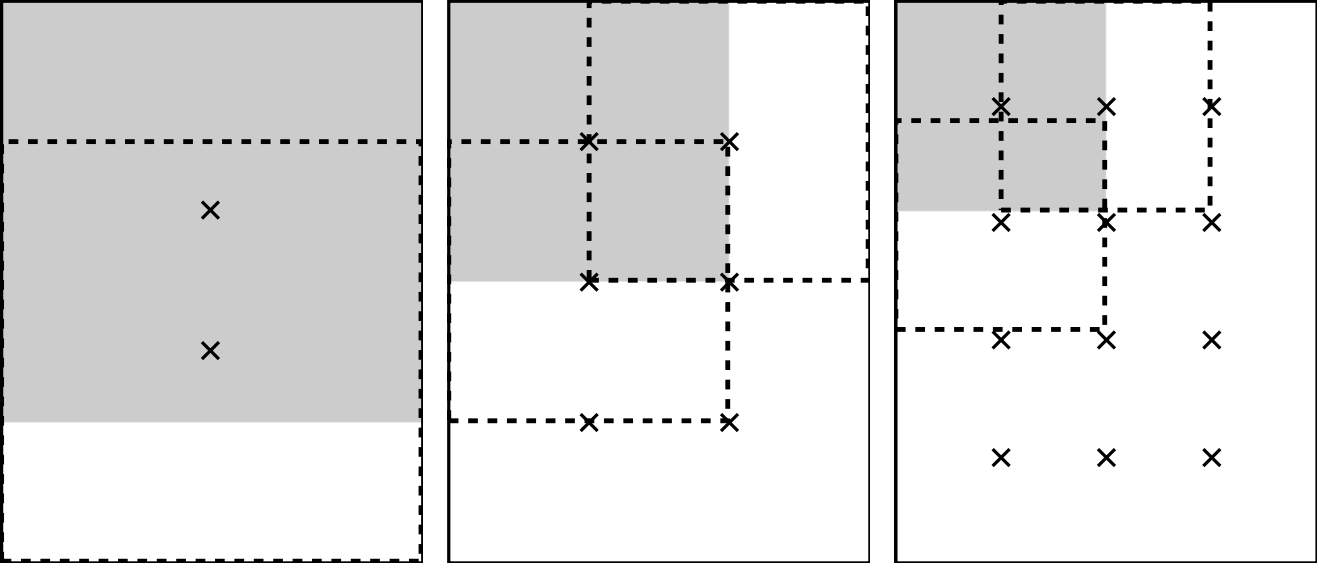
\includegraphics[width=0.6\linewidth]{rmac-regions}
    \caption{Example of regions chosen to extract the \gls{rmac} image descriptor from a \gls{cnn} feature map. \figfrom{tolias2016rmac}.}
    \label{fig:back:rmac-regions}
\end{figure}

\paragraph{\acrlong{rmac}}
Let $\x \in \R^{H \times W \times K}$ the output of a convolutional layer of a pre-trained \gls{cnn} comprised by $K$ feature maps with $H \times W$ spatial resolution, and $\x_i$ the $i$-th feature map.
Given a region $\Reg$ defined over the feature map spatial dimensions, a region descriptor $\f_\Reg$ is obtained by max-pooling along $\Reg$
\begin{equation} \label{eq:back:rmac-region}
\f_\Reg = [\f_{\Reg,1}, \ldots, \f_{\Reg,K}] \qquad \f_{\Reg,i} = \max_{p \in \Reg} \x_i(p) \,,
\end{equation}
where $\x_i(p)$ indicates the activation at a particular spatial position $p$ of the feature map.
Region descriptors are extracted using multiple overlapped squared regions at multiple scales, and region are chosen in order to have an overlap nearest to 40\% (see \ref{fig:back:rmac-regions}).
All the region descriptors are $l_2$-normalized, PCA-whitened% FROM Tolias: (Jégou & Chum, 2012)
, and $l2$-normalized again, and the final \gls{rmac} descriptor is obtained by summing together the post-processed region descriptors and $l2$-normalizing the result.
The obtained descriptor accurately describe multiple local parts of the image at multiple scale and can be computed very efficiently;
in fact, there is no need to crop, resize, and re-feed the image to obtain a multi-scale local description.
Two descriptors are matched using the cosine similarity.

% TODO [FIGURE] RMAC+ substitute figure from gordo2017end with RPN
\begin{figure}
    \centering
    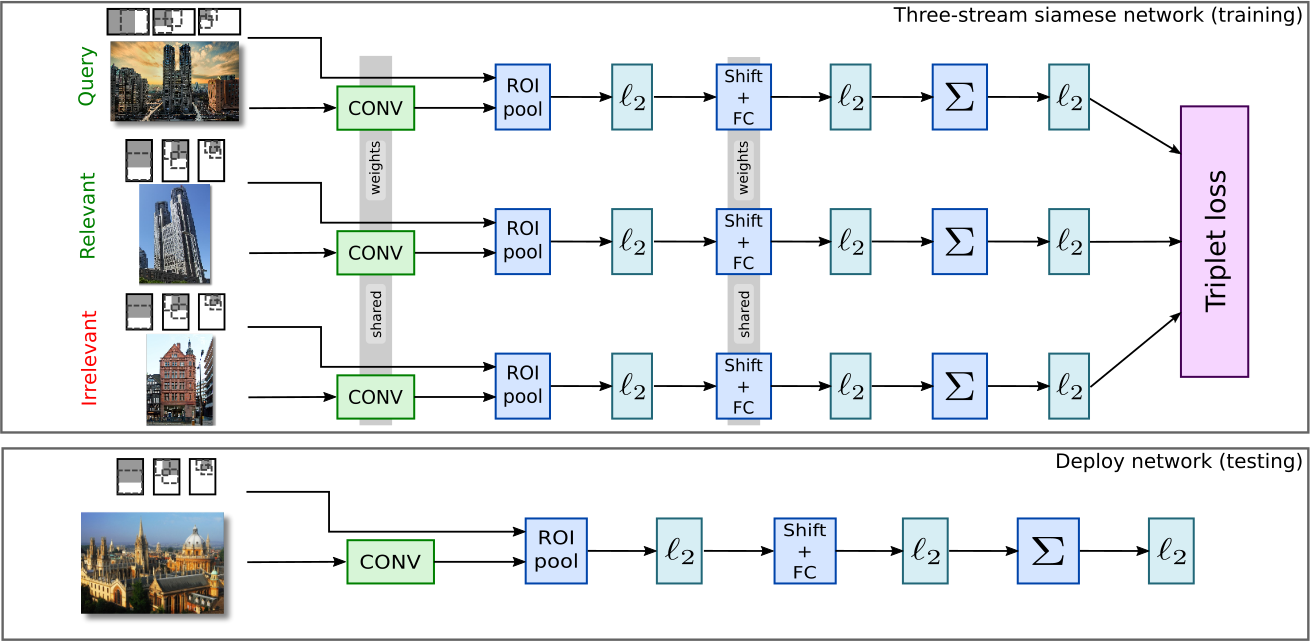
\includegraphics[width=\linewidth]{rmac-trained}
    \caption{Training and deploy pipelines proposed by~\citet{gordo2016deep,gordo2017end} for learning image representations for retrieval. \figfrom{gordo2016deep}.}
    \label{fig:back:rmac-trained}
\end{figure}

\paragraph{Learning Representations for Retrieval}
Representations obtained by transfer learning and their aggregation demonstrated the potential of features extracted by \glspl{cnn}.
However, some of the properties of the representations learnt in classification tasks --- such as robustness to intra-class variability --- are undesirable in some retrieval tasks, e.g.\ instance-level image retrieval.
Succeeding work further improved the state of the art by learning representations directly suited for the task of image retrieval.
\citet{arandjelovic2016netvlad} proposed a differentiable generalization of the VLAD aggregation pipeline called NetVLAD which is eligible to be learned in a neural network framework.
The authors added the NetVLAD module to the last convolutional layer of a pre-trained \gls{dcnn} and fine-tuned the whole pipeline defining a weakly supervised triplet ranking loss.
Similarly, \citet{radenovic2016cnn} fine-tuned a pre-trained \gls{cnn} extracting MAC representations with a siamese loss.
The matching and non-matching couples were chosen in an unsupervised way exploiting a large set of unlabelled landmark photos and an automatic 3D reconstruction system based on local features and geometric consistency.
Of particular interest is the work of \citet{gordo2016deep,gordo2017end}, in which a residual \gls{cnn} equipped with a R-MAC pipeline are fine-tuned with a triplet loss to generate a compact and effective global image descriptor.
Moreover, the authors employed a \gls{rpn} --- a regression model that predicts regions of interest from an image --- to establish the regions aggregated by R-MAC instead of using overlapping grids.
The obtained representations outperform methods based on local features and spatial verification on multiple datasets on both effectiveness and computational efficiency.
\ref{fig:back:rmac-trained} depicts the training and deploy pipelines proposed.

\subsection{Cross-modal Image Retrieval}
%Cross-modal Retrieval

%FROM Picture it:
% Deep Learning and Deep Convolutional Neural Networks (DCNNs) in particular, have recently shown impressive performance on a number of multimedia information retrieval tasks [27, 41, 17]. Deep Learning methods learn representations of data with multiple levels of abstraction. As a result, the activation of the deeper hidden layers has been used in the context of transfer learning and content-based image retrieval [9, 37] as high-level representations of the visual content. Somewhat similarly, distributional semantic models, such as those produced by Word2Vec [33], or GloVe [36], have been found useful in modeling semantic similarities among words by establishing a connection between word meaning and position in a vector space.
Practical applications of \gls{cbir} often require the retrieval system to have more query formulation methods other than \emph{query-by-example}, the most common one being textual search.
Similarly to \glspl{cnn} for visual content representation, \gls{ml} approaches applied to text --- such as Word2Vec~\cite{mikolov2013distributed} and GloVe~\cite{pennington2014glove} --- succeeded to model its semantics and represent it into vector spaces where words meaning are connected with their position in the space.
%In order to perform cross-media retrieval, the two feature spaces (text and images in our case) should be made comparable, typically by learning how to properly map the different media.
Having at hand semantic representations of data coming from different media, in cross-modal retrieval we need to map between them in order to be comparable.
Defining a mapping function is often not trivial, and \gls{dl} approaches shine in learning those mappings leveraging large annotated multi-modal datasets, such as \gls{coco}.
Once the data lie on the same semantic space, we can score and rank items of whichever modality following the same principles applied in the \emph{query-by-example} paradigm.
% This problem has been attempted in different manners so far, which could be roughly grouped into three main variants, depending on whether the mapping is performed into a common latent space (Section 2.1), a textual space (Section 2.2), or a visual space (Section 2.3).
The problem of mapping modalities has led to three main research paths that differ for the chosen destination space for the mapping, that is i) common space, ii) textual space, or iii) visual space approaches.
In the following, we will review some of the recent works on cross-modal retrieval dividing them in this three categories, and we will refer without loss of generality to the case in which we are retrieving images starting from textual queries. %, but the same principles apply to other modalities.

%Textual / visual / common space retrievals
\paragraph{Common Space Approaches}
In common space approaches, the goal is to build a common latent space in which both modalities are mapped into and compared.
%The idea of comparing texts and images in a common latent space has been investigated by means of Cross-modal Factor Analysis and (Kernel) Canonical Correlation Analysis in [7, 15].
% nothing here..
%In a similar vein, Corr-AE was proposed for cross-modal retrieval, allowing the search to be performed in both directions, i.e.\ from text-to-image and vice versa [12].
% The idea is to train two autoencoders, one for the image domain and another for the textual domain, imposing restrictions between the two.
In \cite{ngiam2011multimodal,feng2014cross}, the authors propose to use autoencoders, i.e.\ neural network models that learn to encode its input by creating a low-dimensional code and by reconstructing its input starting from that code;
a common space is created by imposing a correlation between the code of two autoencoders, one for the image domain and another for the textual domain.
%Similarly, in \cite{kiros2014unifying} the authors propose an encoder-decoder architecture, in which the encoder part, formed by a LSTM (for textual input) and a CNN (for visual input), is trained to project both inputs into near points in a common multimodal space, and the decoder part generates new text from a point in this new space.
\citet{kiros2014unifying} defined a multi-modal encoder-decoder architecture, in which text and images are encoded in a common space by two branches respectively implemented with an \gls{lstm} and a \gls{cnn};
the encoders are trained to place coupled inputs in near points in the common space.
%As will be seen, one of the architectures we are presenting in the following (S-Text2Vis, Section 3.2) bears resemblance to one of the architectures investigated in [12], the so-called Correspondence full-modal autoencoder (which is inspired by the multimodal deep learning method [34]).
% However, the two networks have a fundamental difference, since the Correspondence full-modal autoencoder takes examples from both media as the inputs. TODO move to chapter
%
%The DeViSE [13] method jointly trains a pretrained instance of the convolutional neural network of [27] (with its last layer replaced with a linear mapping into the final embedding space), and a textual embedding space pre-trained as a skip-gram model [33].
% Even though DeViSE uses a final space which is of the same size of the textual space, the pre-trained word embeddings are only used as initial parameters and then they are adapted jointly with visual embeddings during the training.
% The training is made on image and label pairs, where the labels are not a full description of the scene, indicating only the presence of certain entities in the image.
In \cite{frome2013devise}, the authors proposed a \gls{devise} model in which a pre-trained \gls{cnn} (AlexNet) and a pre-trained skip-gram textual embedding model (Word2Vec) are adapted to a common space and jointly fine-tuned on image and label pairs.

Common space approaches allows to retrieve items in both modalities starting from a query in whichever modality, e.g.\ is it possible to retrieve images by text or texts by image.
However, depending on the needs of the retrieval system, a particular modality may be the preferred way to represent your data in the search database, and a common space projection of all the database may not be viable.
Consider for example an existing textual document search engine which would like to implement image search by keyword without building a separate image retrieval system.
In this scenarios, mapping a query into an existing space may result in a suitable solution.
In the next paragraphs, we will briefly review relevant works that exploit this strategy and leverage an existing textual or visual space to enable cross-media image retrieval.

\paragraph{Search in Textual Space}
%The BoWDNN method [1] trains a deep neural network to map images directly into a \acrfull{bow} space, where the cosine similarity between BoWs representations is used to generate the ranking.
In \cite{bai2014bag}, a \acrfull{bow} space representing text is used as target space, and a deep neural network called BowDNN is proposed to map images into \glspl{bow}s representations that are then compared with cosine similarity.
% Somehow similarly, a dedicated area of related research is focused on generating captions describing the salient information of an image (see, e.g., [22, 11, 44]).
Many other works focus on mapping images directly to a textual description, i.e.\ producing a caption of the image describing its salient content~\cite{vinyals2015show,karpathy2015deep,fang2015captions}.
%The m-RNN method [31] trains a multimodal recurrent neural network to generate a caption description for a given image.
% The model consists of a recurrent sub-network (operating on text data) and a convolutional sub-network (operating on image data) which combine into a multimodal layer where the recurrent state interacts with the image representation.
In \cite{mao2014deep}, a multi-modal recurrent neural network (m-RNN) is proposed to generate captions for a given image;
an image representation is extracted by a convolutional sub-network and combined with each the hidden state of a recurrent network to predict the sequence of words comprising the caption.
%In [30], authors propose m-CNN, a multimodal architecture in which convolutions are used on both the image and textual inputs to directly output a match score between them.
% Models like m-CNN, which do not explicitly learn a projection but a distance function on a latent projection, are not fit for retrieval on large collections.
% Given a query, such models need to perform a forward pass through the network for every image in the collection in order to compute the distances.
% This entails a much higher cost with respect to traditional metrics, such as the Euclidean distance or the cosine similarity. TODO move to chapter
%The ConSE [35] method adopts a very simple approach, inspired by DeViSE, that uses the classification labels of the convolutional neural network of [27] to select and combine, by their classification probability, the set of textual embeddings related to the top assigned labels.
Inspired by \gls{devise}, \citet{norouzi2013zero} proposed the ConSE method, in which the image is classified by a pre-trained AlexNet, and a combination of textual embeddings is produced leveraging the most probable labels and its degree of confidence assigned by the network.

\paragraph{Search in Visual Space}
Methods that maps a textual query in a visual space are less explored and thus object of our investigation in this thesis (see \ref{ch:text2vis}).
One of the most relevant and recent work in this subfield is Word2VisualVec \cite{dong2018predicting}, in which a deep \gls{mlp} is trained to predict visual features extracted from a pre-trained \gls{cnn} starting from a textual encoding obtained by a combination of Word2Vec representations.
We argue that this kind of solution is suitable in the cases in which we need to access a large dataset of images for which visual features have already been extracted and indexed, and we want to exploit the same data structures to perform a textual search.
Being the visual space independent from a particular language, multiple text-to-visual-code models can be trained and deployed to support textual search in multiple languages without the need to replicate data representations.

%Our Text2Vis variants belong to this group where, to the best of our knowledge, the only other proposal up to now is a method dubbed Word2VisualVec [10], which was reported just very recently. There are some fundamental points where their method and ours differ, though. Word2VisualVec takes combinations of Word2Vec-like vectors as a starting point, thus reducing the dimensionality of the input space, whereas we directly take the \acrlong{bow} vector encoding of the textual space as the input (S-Text2Vis), or learn the word embeddings (D-Text2Vis, Section 3.3) during the training process, as we did not observe any improvement in pre-training the textual part. Moreover, Word2VisualVec builds a deep regressor on top of the textual representation that are aggregations of word embeddings, which thus discard word order information. Contrarily, we observed that, when disregarding word order, yet a shallow regressor (S-Text2Vis) produces effective mappings of textual vectors into the visual space. We also observed that taking word order into account helps to improve results (D-Text2Vis and W&D-Text2Vis, Section 3.4). TODO move to chapter


\subsection{Evaluation Metrics}
\label{subsec:back:ir-metrics}
The image retrieval problem is not so different from classical textual information retrieval problem, thus it borrows from it much of the terminology, formulations and evaluation metrics.
% accuracy, computational cost, memory consumption
The main aspects to be considered in the evaluation of a retrieval system are its accuracy and its computational \& memory consumption in both the off-line and on-line stages.
While measuring computational and memory resources in this scenario is straightforward, researches dedicated multiple metrics to measure the accuracy of a retrieval system.
In the following paragraphs, we will introduce the notation and some of the conventionally used evaluation metrics.

Given a collection of images $\X$ and a query image $\q$, the goal is to retrieve the set of images $\X_q \subset \X$ relevant to $\q$.
In the feature-based approach, an image is represented by its feature vector $\x$, and a similarity $s(\cdot)$ (or distance $d(\cdot)$) function is defined to compare two feature vectors.
This function permits to assign a similarity score (or a distance) to each element of our search collection and to sort them based on their relevancy to the query.
Since the top elements on the candidate list are the ones to be most plausible to be consumed by the user, many of the evaluation metrics for measuring the accuracy of a retrieval system are thought to evaluate the goodness of the initial part of the results list.

Assume $\X$ %$= {\x_1, \ldots, \x_N}$
is a collection of $N$ elements, $\q$ a query, $\Y^{\star}_{\q} \subset \X$ the subset of $\X$ relevant to $\q$, and $\Y_{\q}$ the retrieved candidate set to be evaluated.
% = {\y_1, \ldots, \y_N} \subset \{0,1\}^N$ a set of $N$ indicator variables where $\y_i = 1$ if $\x_i$ is relevant for $\q$, 0 otherwise.
% PR
\paragraph{Precision and Recall}
With \emph{precision}, we refer to the fraction of retrieved samples that are relevant to the query
\begin{equation} \label{eq:back:precision}
\text{Precision} = \frac{|\Y_{\q} \cap \Y^{\star}_{\q}|}{|\Y_{\q}|} \,,
\end{equation}
where $|\cdot|$ indicates the cardinality of a set.
We refer to the fraction of relevant samples actually retrieved as \emph{recall}
\begin{equation} \label{eq:back:recall}
\text{Recall} = \frac{|\Y_{\q} \cap \Y^{\star}_{\q}|}{|\Y^{\star}_{\q}|} \,.
\end{equation}

A trade-off between precision and recall is often tuned on deployment;
the system may be tuned to retrieve only objects similar to the query with high confidence thus achieving high precision, but may leave behind some relevant samples and obtaining a low recall.
Viceversa, a less stringent retrieval has a high recall, but more retrieved samples may not be relevant to the query, decreasing the precision of the system.

% mAP
\paragraph{\acrlong{ap}}
The \emph{\acrfull{ap}} metric is commonly used to evaluate a retrieval system independently from the particular configuration of precision-recall.
Similarly to the \acrfull{auc} of ROC plots --- discussed in \ref{subsec:back:classif-eval} --- the \gls{ap} represent the area under the precision-recall curve and is computed as
\begin{equation} \label{eq:back:ap}
    \text{AP} = \sum_r p(r)\,,
\end{equation}
where $r$ is the set of possible recall values that can be achieved, e.g.\ varying the maximum number of elements to be retrieved or the threshold on the scores of the retrieved samples.
When multiple queries are considered for evaluation, the \emph{\acrfull{map}} is usually reported, which is the mean of the \glspl{ap} obtained from each query.

%nDCG
\paragraph{\acrlong{dcg}}
The \emph{\acrfull{dcg}}~\cite{jarvelin2002cumulated} is conventionally used when multiple level of relevancy are available for samples in the groundtruth.
Its aim is to penalize highly relevant samples in the bottom part of the results;
to do so, usually a logarithmic weighting scheme is adopted to assign a decreasing importance to samples in the lower part of the search results.
The \gls{dcg} at the rank position $n$ is defined as
\begin{equation} \label{eq:back:dcg}
    \text{DCG}@n = \sum_{i=1}^n \frac{2^{r_i} - 1}{\log_2(i + 1)} \,,
\end{equation}
where $r_i$ is a positive scalar representing the relevance of the $i$-th retrieved sample.
In the case rankings can have ties, the \gls{tdcg}~\cite{mcsherry2008computing} is used, defined as:
%
\begin{equation}
\text{TDCG}@n = \sum_{i=1}^{m}\left(\left(\frac{1}{n_i}\sum_{j=t_i+1}^{t_{i+1}}2^{rel_i}-1\right)\sum_{j=t_i+1}^{\min(t_{i+1},k)}\frac{1}{\log_2(i+1)}\right)
\end{equation}
%
where $m$ is the number of group of ties in the ranking of the first $n$ results, $n_i$ indicates the number of tied result in the $i$-th group, $t_i$ indicates the starting position of each tied group.
The $TDCG$ is derived from $DCG$ by observing that the average gain for a position in a group of tied results is the average of the gain of such tied results.
The $TDCG$ is obviously equivalent to $DCG$ in the case there are no ties in the results.

% NDCG is divided by a normalization factor to ensure the metric is in the $[0,1]$ range.

% R@K
\paragraph{\acrlong{r@k}}
The \acrfull{r@k} is the recall metric when considering only the top-K results of the groundtruth as relevant.
It is conventionally used to compare two rankings in absence of an explicit relevancy labelling of the groundtruth.
Assuming $\Y^{\star}_{\q, K}$ the set of samples relevant to $\q$ truncated at the $K$-th element, and $\Y_{\q,K}$ the top-$K$ retrieved elements to be evaluated, the \gls{r@k} is defined as
\begin{equation} \label{eq:back:r@k}
    R@K = \frac{|\Y^{\star}_{\q, K} \cap \Y_{\q,K}|}{K} \,.
\end{equation}

%medR
\paragraph{\acrlong{medR} and \acrlong{mrr}}
These metrics are particularly useful when evaluating rankings in which there is only one object in the database relevant to the query that need to be retrieved.
Cross-modal retrieval with coupled datasets is an examples in which this condition applies: using as query one modality of a sample, a common approach is to evaluate how well the system is able to retrieve the same sample in the different modality.
Given multiple queries, the \acrfull{medR} is the median of the positions of the relevant objects in the rankings, one per query,
% MRR
while the \acrfull{mrr} is the mean of the reciprocals of the same quantities.

% TODO move indexing in chapter
%\subsection{Image Indexing}
%\label{sec:back:indexing}
%kNN schemes
%Permutation-based representations
%Deep Permutations

%Datasets & Evaluation Metrics

\section{Datasets}
\label{sec:back:datasets}
In this section, we will list the dataset --- either publicly available or collected --- used directly or indirectly in the experiments presented in this work.

\subsection{Classification Datasets}

\paragraph{\acrfull{ilsvrc} 2012~~\cite{russakovsky2015imagenet}}
The \acrfull{ilsvrc} 2012 dataset is composed by a large set of images of general objects collected for evaluating algorithms for large-scale visual object recognition.
It is a subset of roughly 1.3 million images taken from the larger ImageNet\footnote{\url{http://www.image-net.org}} database --- a big collection of images labelled and organized following the hierarchical categorization of WordNet.
Images are assigned a single label chosen from the 1,000 classes selected for the competition, spanning general objects, animals, etc.
Each class has roughly 1,000 images in the training set (the number oscillates between 700 and 1,300), and exactly 50 and 100 images respectively in the validation and test set, for a total of 1,281,167 images for the train set, 50,000 for the validation set, and 100,000 in the test set.
Only the training and validation sets are publicly available.

\paragraph{Places205~\cite{zhou2014learning}}
The Places205 dataset is composed by roughly 2.5 million images collected from image search engines labelled with 205 semantic scene categories and attributes representing visual environments all over the world.
It is a subset of the bigger Places dataset~\cite{zhou2016places}.

\paragraph{PKLot~\cite{de2015pklot}}
The PKLot dataset is an car parking occupancy detection dataset comprised by 12,417 images of 3 parking lots, named UFPR04, UFPR05, and PUC, took in different days and weather conditions.
The images have been segmented in 695,899 images of parking spaces by cropping along the rotated rectangles delimiting each parking space and rotating back the cropped patches in vertical or horizontal position.
Each segmented image is labelled with the vacancy status of the slot, which can be either occupied or vacant.

\paragraph{CNRPark+EXT~\cite{amato2016car,amato2017deep}}
The CNRPark+EXT dataset is a car parking occupancy detection dataset collected during this thesis from the parking lots of the campus of the National Research Council (CNR) in Pisa.
It is comprised by roughly 150,000 images of parking spaces taken from 9 smart cameras with different view-points, in different days with different weather and light conditions, and includes occlusion and shadow situations that make the occupancy detection task challenging.
More details about the CNRPark-EXT dataset will
be given in \ref{ch:miniaturization}.

\paragraph{Twitter Testing Dataset~\cite{you2015robust}}
The Twitter Testing Dataset is a dataset for image sentiment analysis composed by 1269 images labelled with crowd-sourcing (Amazon Mechanical Turk) following a binary positive/negative sentiment polarity scheme.
Each image has been annotated as positive or negative by five workers, and three different subsets have been created, respectively comprised by images where 5 workers agree on the sentiment of the image (5-agree, 882 images), where at least 4 workers agree (4-agree, 1,116 images), and where at least 3 workers agree (3-agree, whole set of images).

\paragraph{\acrfull{t4sa}~\cite{vadicamo2017cross}}
The \acrlong{t4sa} dataset is a large-scale weakly-labelled dataset for sentiment analysis collected during this thesis to evaluate the weakly-labelled cross-media training procedure for image classifiers presented in \ref{ch:cross-media}.
It is comprised by 904,395 tweets and their corresponding 1,473,394 images (each tweet has one or more images);
tweets have been collected from the 5\% random stream of global tweets provided by the Twitter APIs keeping only tweets in english with at least five words and at least one image.
Each tweet is associated with a three-way sentiment polarity (positive/neutral/negative sentiment) predicted by performing textual sentiment polarity prediction.
More details are available in \ref{ch:cross-media}.

\subsection{Retrieval Datasets}

\paragraph{INRIA Holidays~\cite{jegou2008hamming}}

The INRIA Holidays image set is an image retrieval dataset comprised by 1491 high-resolution holidays photos containing various scenes types.
The authors chose 500 queries and manually selected from the set the images relevant for each query.
A frequently used variant of this dataset is the one augmented with \emph{MIRFlickr1M}, a distractor set of 1 million images collected by the Flickr service;
we refer to this new dataset as \emph{Holidays-MIRFlickr1M}.

\paragraph{Oxford Buildings~\cite{philbin2007object}}
The Oxford Buildings dataset, also known as \emph{Oxford5k}, is an image retrieval dataset comprised by 5,062 images of various buildings present in Oxford.
The set is composed by photos of 11 famous buildings plus distractor images collected from Flickr.
For each building, five queries are specified with bounding boxes delimiting the building we are interested in retrieving, for a total of 55 query images.
For each query, images of the search set are assegned with one of the following four labels:
\begin{itemize}
    \item \emph{ok} --- if the image contains a clear look of the building in the query;
    \item \emph{good} --- if more than 25\% of the building is clearly visible;
    \item \emph{junk} --- if less than 25\% of the building
is visible, or there is a very high level of occlusion or dis-
tortion;
    \item \emph{absent} --- if the building is not present.
\end{itemize}
In this work, we will adopt the version of this dataset augmented with a distractor set of 100k images collected from Flickr, and we will refer to it as \emph{Oxford-Flickr100k}.

% \paragraph{Paris~\cite{philbin2008lost}}
% \paragraph{Flickr100k and Flickr1M ~\cite{philbin2007object}}

\paragraph{\acrfull{coco}~\cite{lin2014microsoft}}

The Microsoft \acrfull{coco} dataset is a collection of images  for large-scale object detection, segmentation, and captioning.
it is comprised by 2,500,000 labeled object instances belonging to 91 common object categories in 328,000 images.
Each image is associated with an instance-level pixel-wise segmentation of the object instances it depicts and five captions describing the whole images.
This dataset is particularly adopted also in cross-modal retrieval due to its large scale and the presence of captions, and we will use it to compare to existing cross-modal retrieval approaches in \ref{ch:text2vis}.

\subsection{Others}

\paragraph{NIPS Adversarial Attacks and Defences Competition DEV set~\cite{kurakin2018adversarial}}
The NIPS Adversarial Attacks and Defences Competition DEV set is comprised by 1,000 images that do not belong to the \gls{ilsvrc}'12 subsets but share the same label space, i.e.\ are labelled with one of the same 1,000 label used in \gls{ilsvrc}.
This set has been released in the context of the NIPS Adversarial Attacks and Defences Competition on Kaggle to let participants work with pre-trained \gls{ilsvrc} classifiers using images not involved in their training process.
In particular, the set is devoted to generate adversarial examples for image classifiers, i.e.\ maliciously manipulated images the lead a classifier to misbehave.
More details are available in \ref{ch:adversarial} in which we use this set of images to evaluate a detection scheme for adversarial attacks.
